\subsection{Interfaces} %     5.3.1 Interfaces

\change[inline]{Create wireframes, as described on page 439, for every interface
the artists will need to create. Each wireframe should include a description of
how each interface feature functions. Make sure you detail out the various
states for each interface.}

% \urgent{NO OLVIDES AÑADIR LA DESCRIPCIÓN DE CADA ELEMENTO DE CADA INTERFAZ}

\subsubsection{Modo menú principal}
\begin{figure}[H]
    \centering
    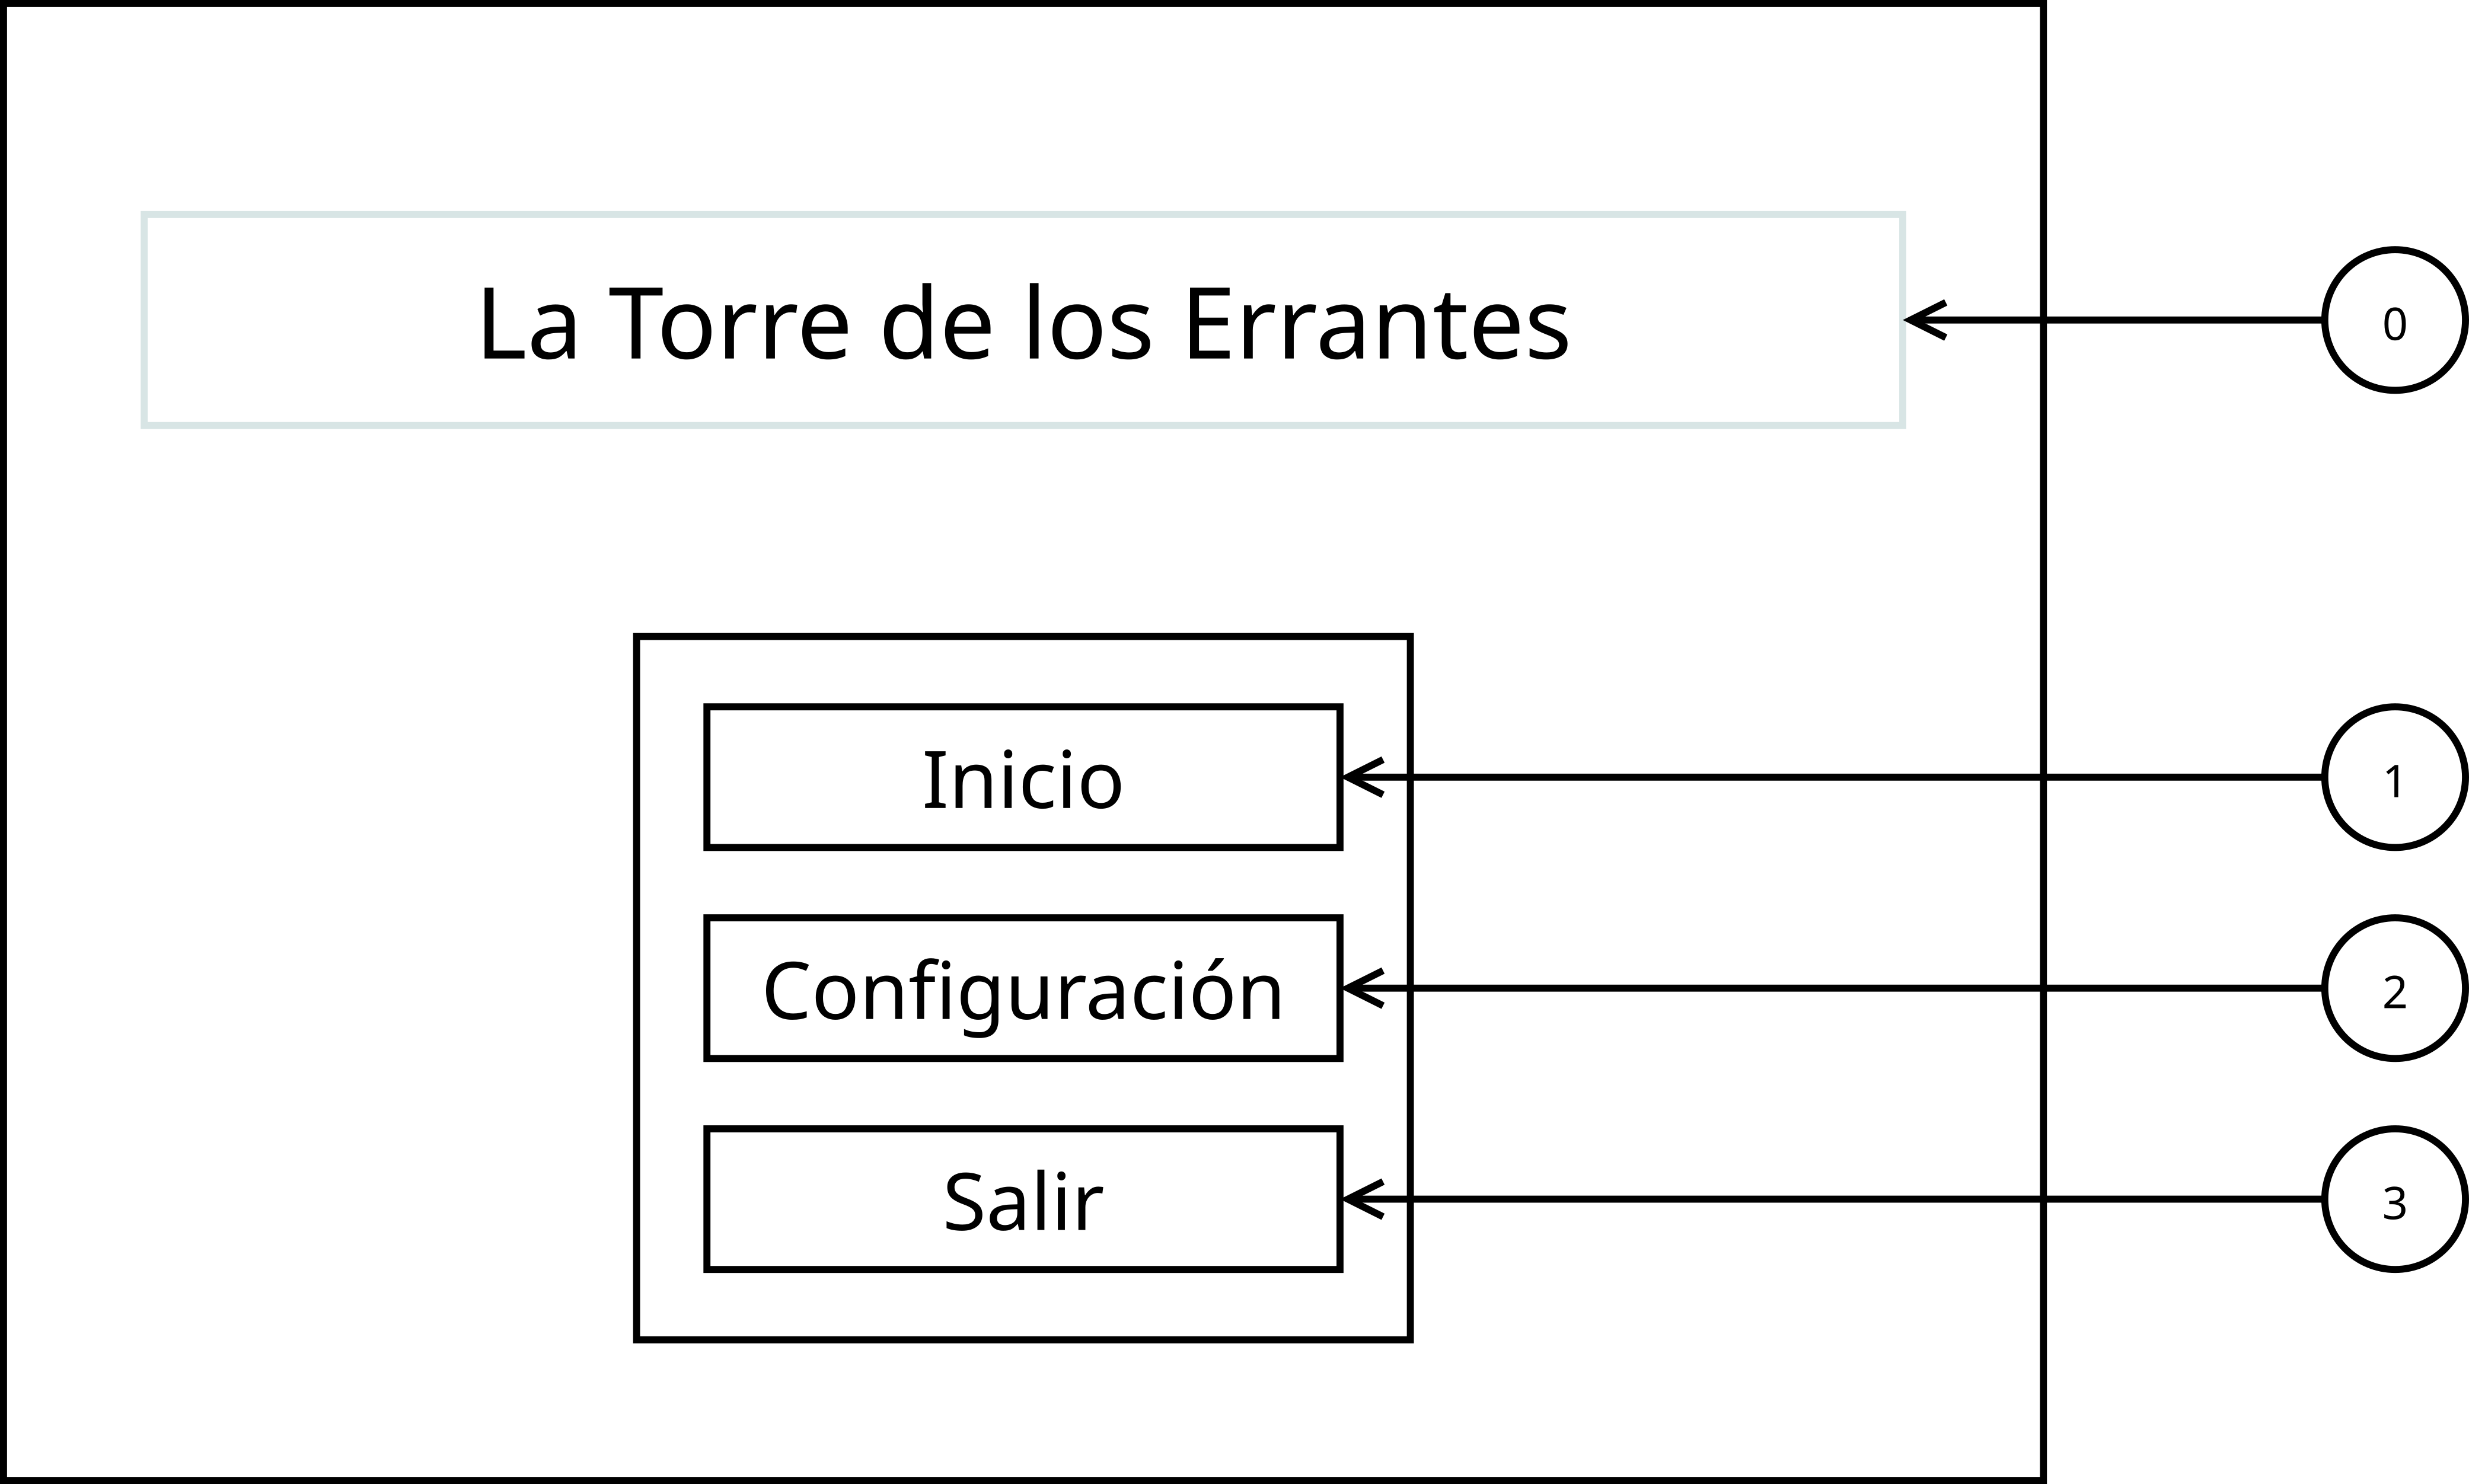
\includegraphics[width=0.6\textwidth]{5-Cuerpo/Chapter5/5.5/I1.png} %
    \caption{Interfaz del menú principal}
    \label{fig:Interface_Menu_Principal}
\end{figure}
\begin{enumerate}\setcounter{enumi}{-1}
    \item \textbf{Nombre del juego}: Se mostrará el título del juego en la
    pantalla de inicio.
    \item \textbf{Botón de inicio}: Se usará este botón para pasar al menú de
    selección de perfil y así iniciar el juego como tal.
    \item \textbf{Botón de configuración}: Se usará este botón para pasar al
    menú de configuración general.
    \item \textbf{Botón de salida}: Se usará este botón para terminar con la
    ejecución del juego y salir así de éste.
\end{enumerate}

\subsubsection{Modo selección de perfil}
\begin{figure}[H]
    \centering
    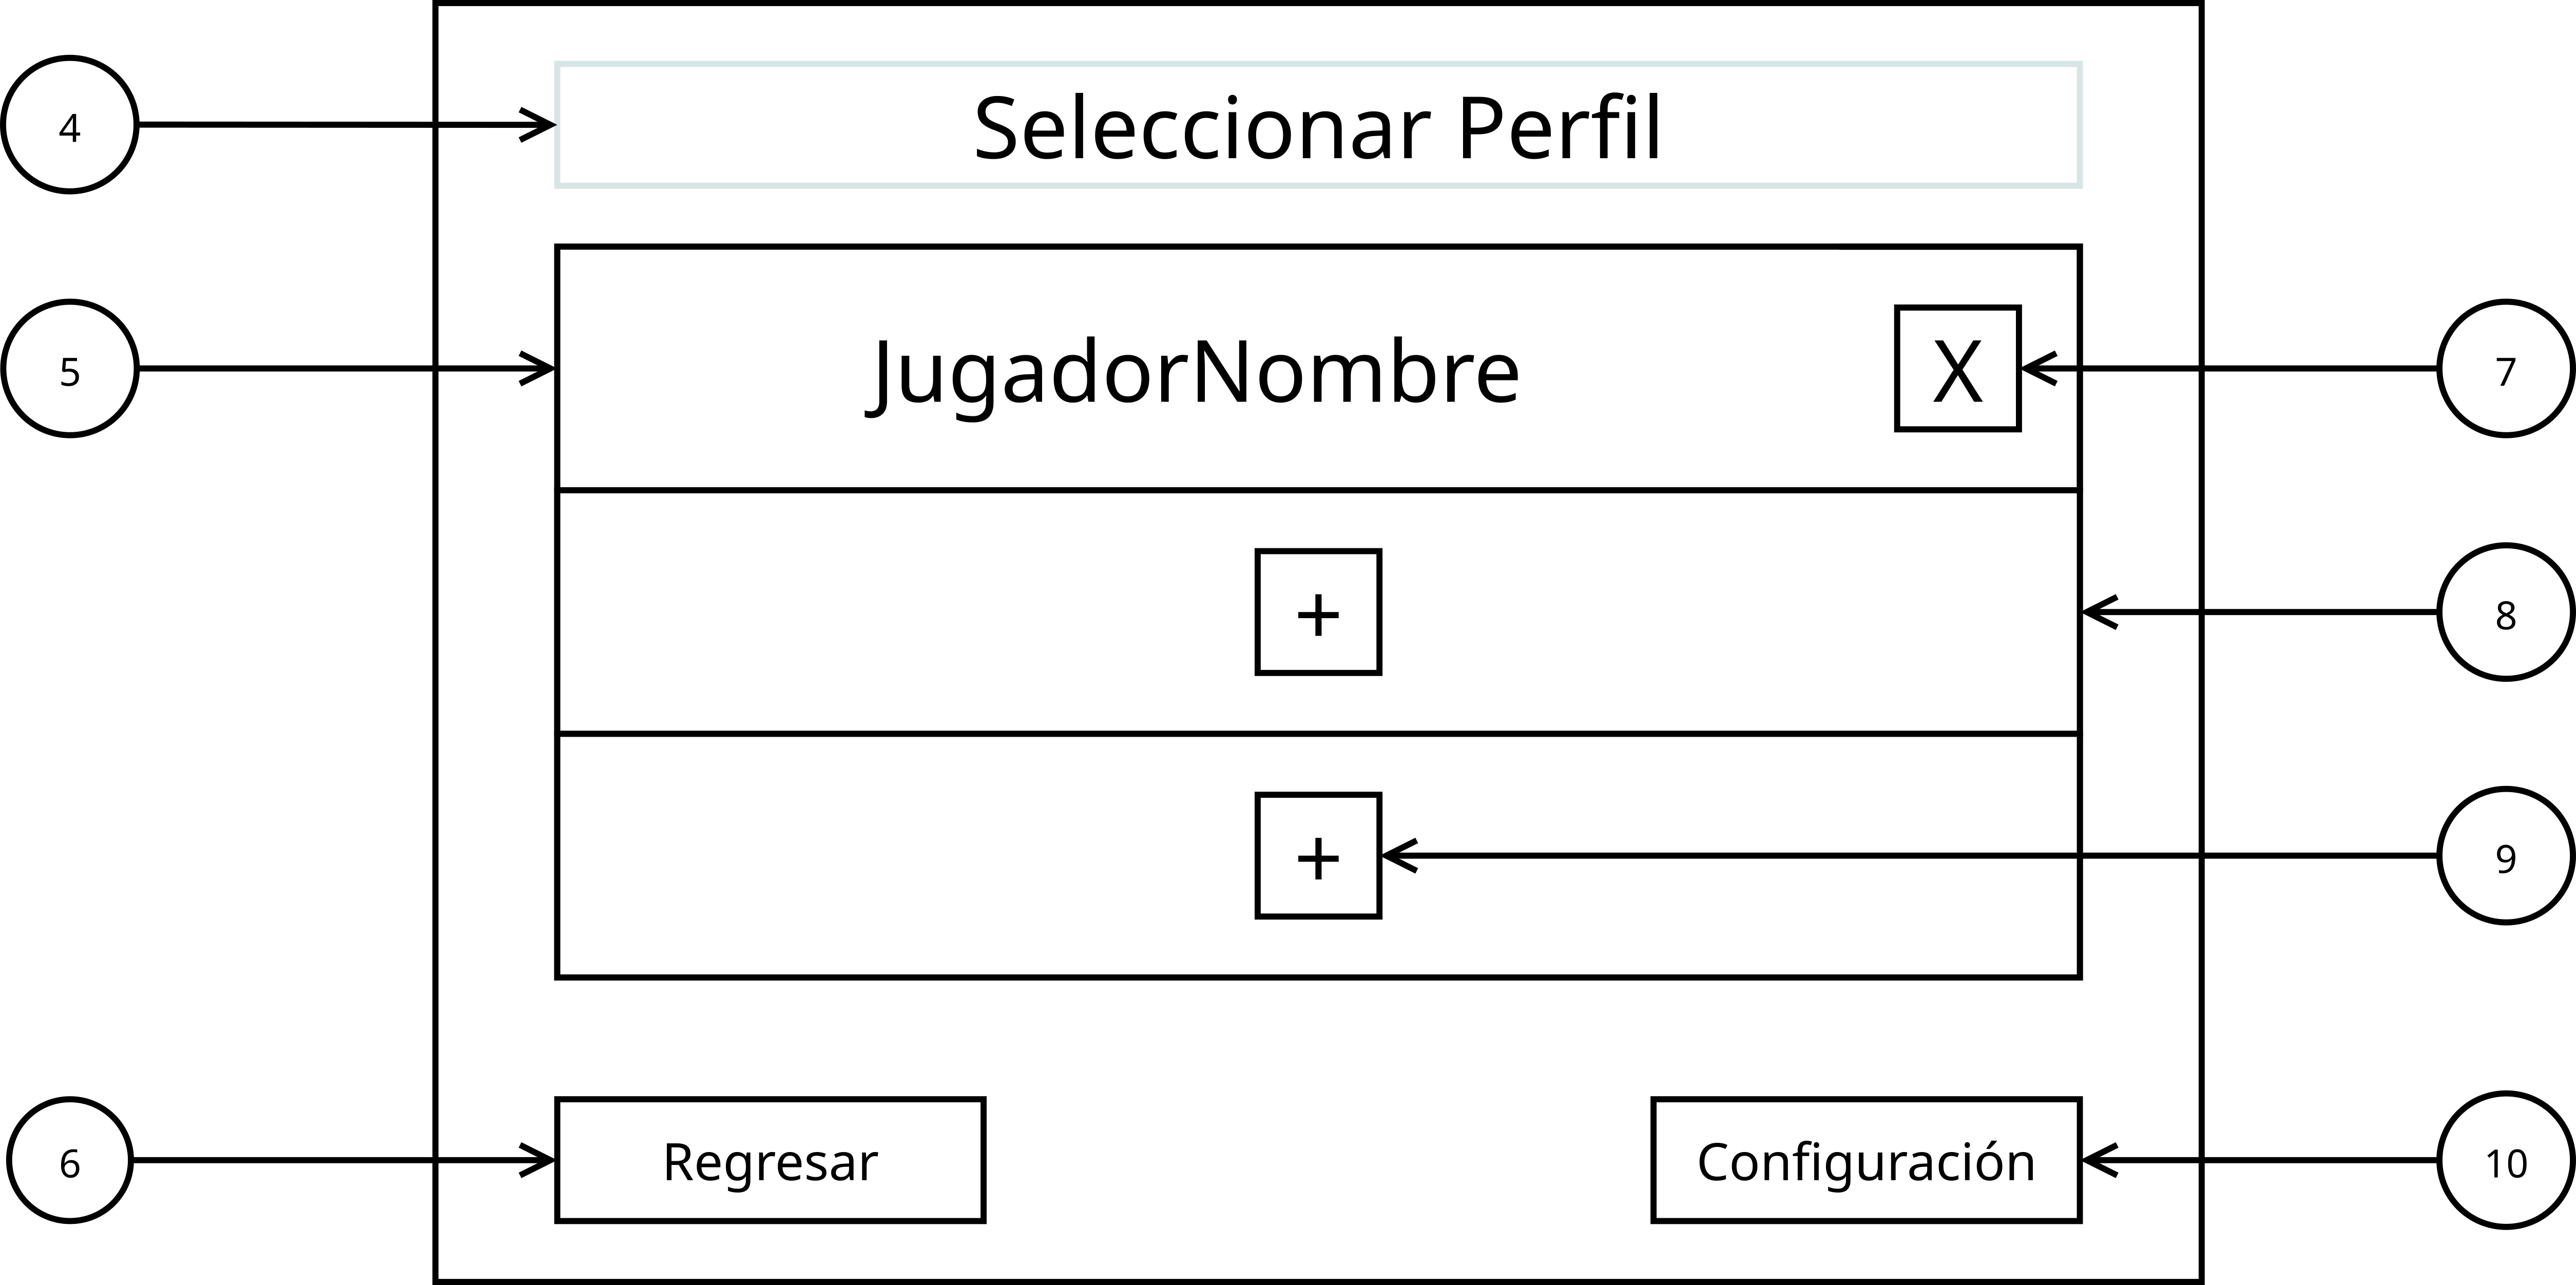
\includegraphics[width=0.6\textwidth]{5-Cuerpo/Chapter5/5.5/I2.png} %
    \caption{Interfaz del menú de selección de perfiles}
    \label{fig:Interface_Seleccion_Perfil}
\end{figure}
\begin{enumerate}\setcounter{enumi}{3}
    \item \textbf{Nombre de la interfaz}: Se muestra el nombre de la interfaz y
    modo actual.
    \item \textbf{Información de perfil}: Se mostrará el nombre de aquellos
    perfiles que ya hayan sido creados. Al darle click a este elemento se pasará
    a al menú de visualización de perfil.
    \item \textbf{Botón de regreso}: Este botón permitirá volver a la interfaz
    anterior a la actual; o mejor dicho, a la interfaz desde la cual se accedió
    a la actual.
    \item \textbf{Eliminar perfil}: Se dará la posibilidad de eliminar los datos
    de un perfil ya creado.
    \item \textbf{Espacio de perfil}: La interfaz mostrará también los espacios
    de perfil que todavía no se estén usando para poder permitir crear uno nuevo
    estos.
    \item \textbf{Crear perfil}: Este botón permitirá la creación de un nuevo
    perfil dentro de un espacio no ocupado.
    \item \textbf{Botón de configuración}: Este botón llevará a la interfaz de
    configuración general del juego.
\end{enumerate}

\subsubsection{Modo perfil}
\begin{figure}[H]
    \centering
    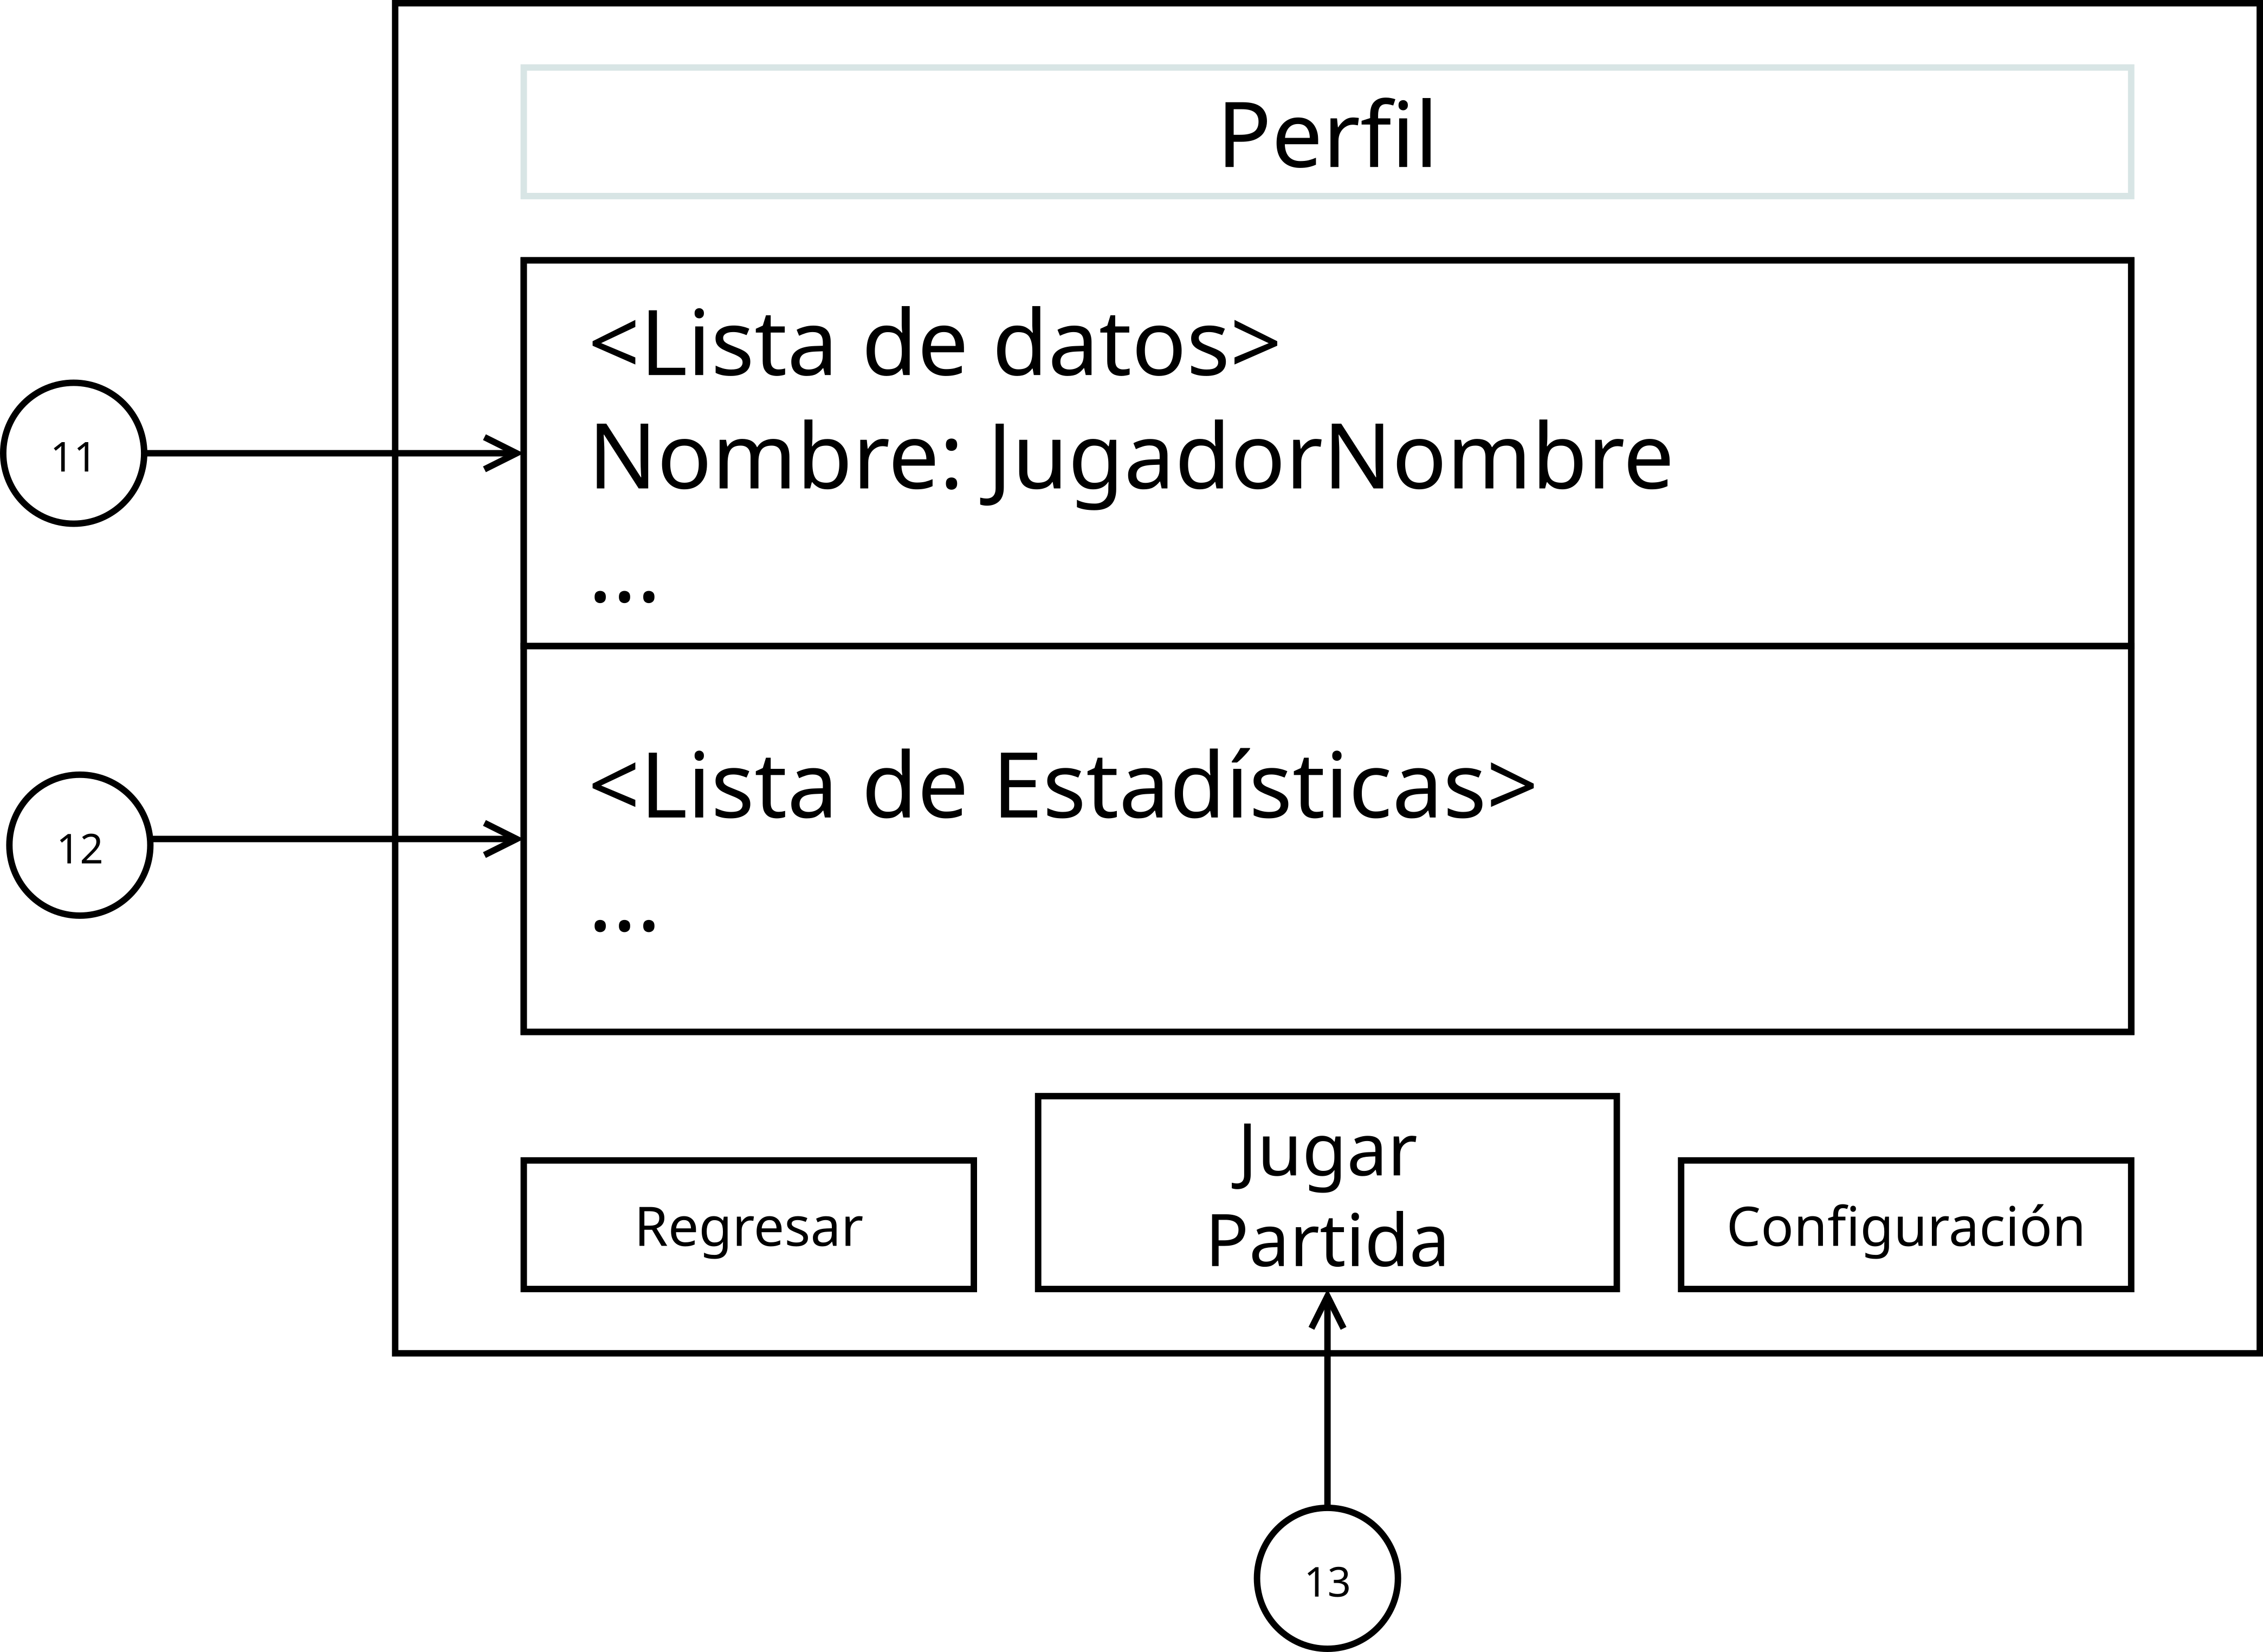
\includegraphics[width=0.6\textwidth]{5-Cuerpo/Chapter5/5.5/I3.png} %
    \caption{Interfaz de visualización de perfil}
    \label{fig:Interface_Perfil}
\end{figure}
\begin{enumerate}\setcounter{enumi}{10}
    \item \textbf{Bloque de datos generales del perfil}: En este espacio se
    mostrarán los datos generales del perfil como lo es el nombre del jugador.
    \item \textbf{Bloque de estadísticas del perfil}: En este espacio se
    mostrarán las estadísticas asociadas al perfil como tal.
    \item \textbf{Botón de inicio del juego}: Para poder empezar una nueva
    partida, se pulsará este botón con el fin de ir al menú de configuración de
    partida.
\end{enumerate}

\subsubsection{Modo configuración de partida}
\begin{figure}[H]
    \centering
    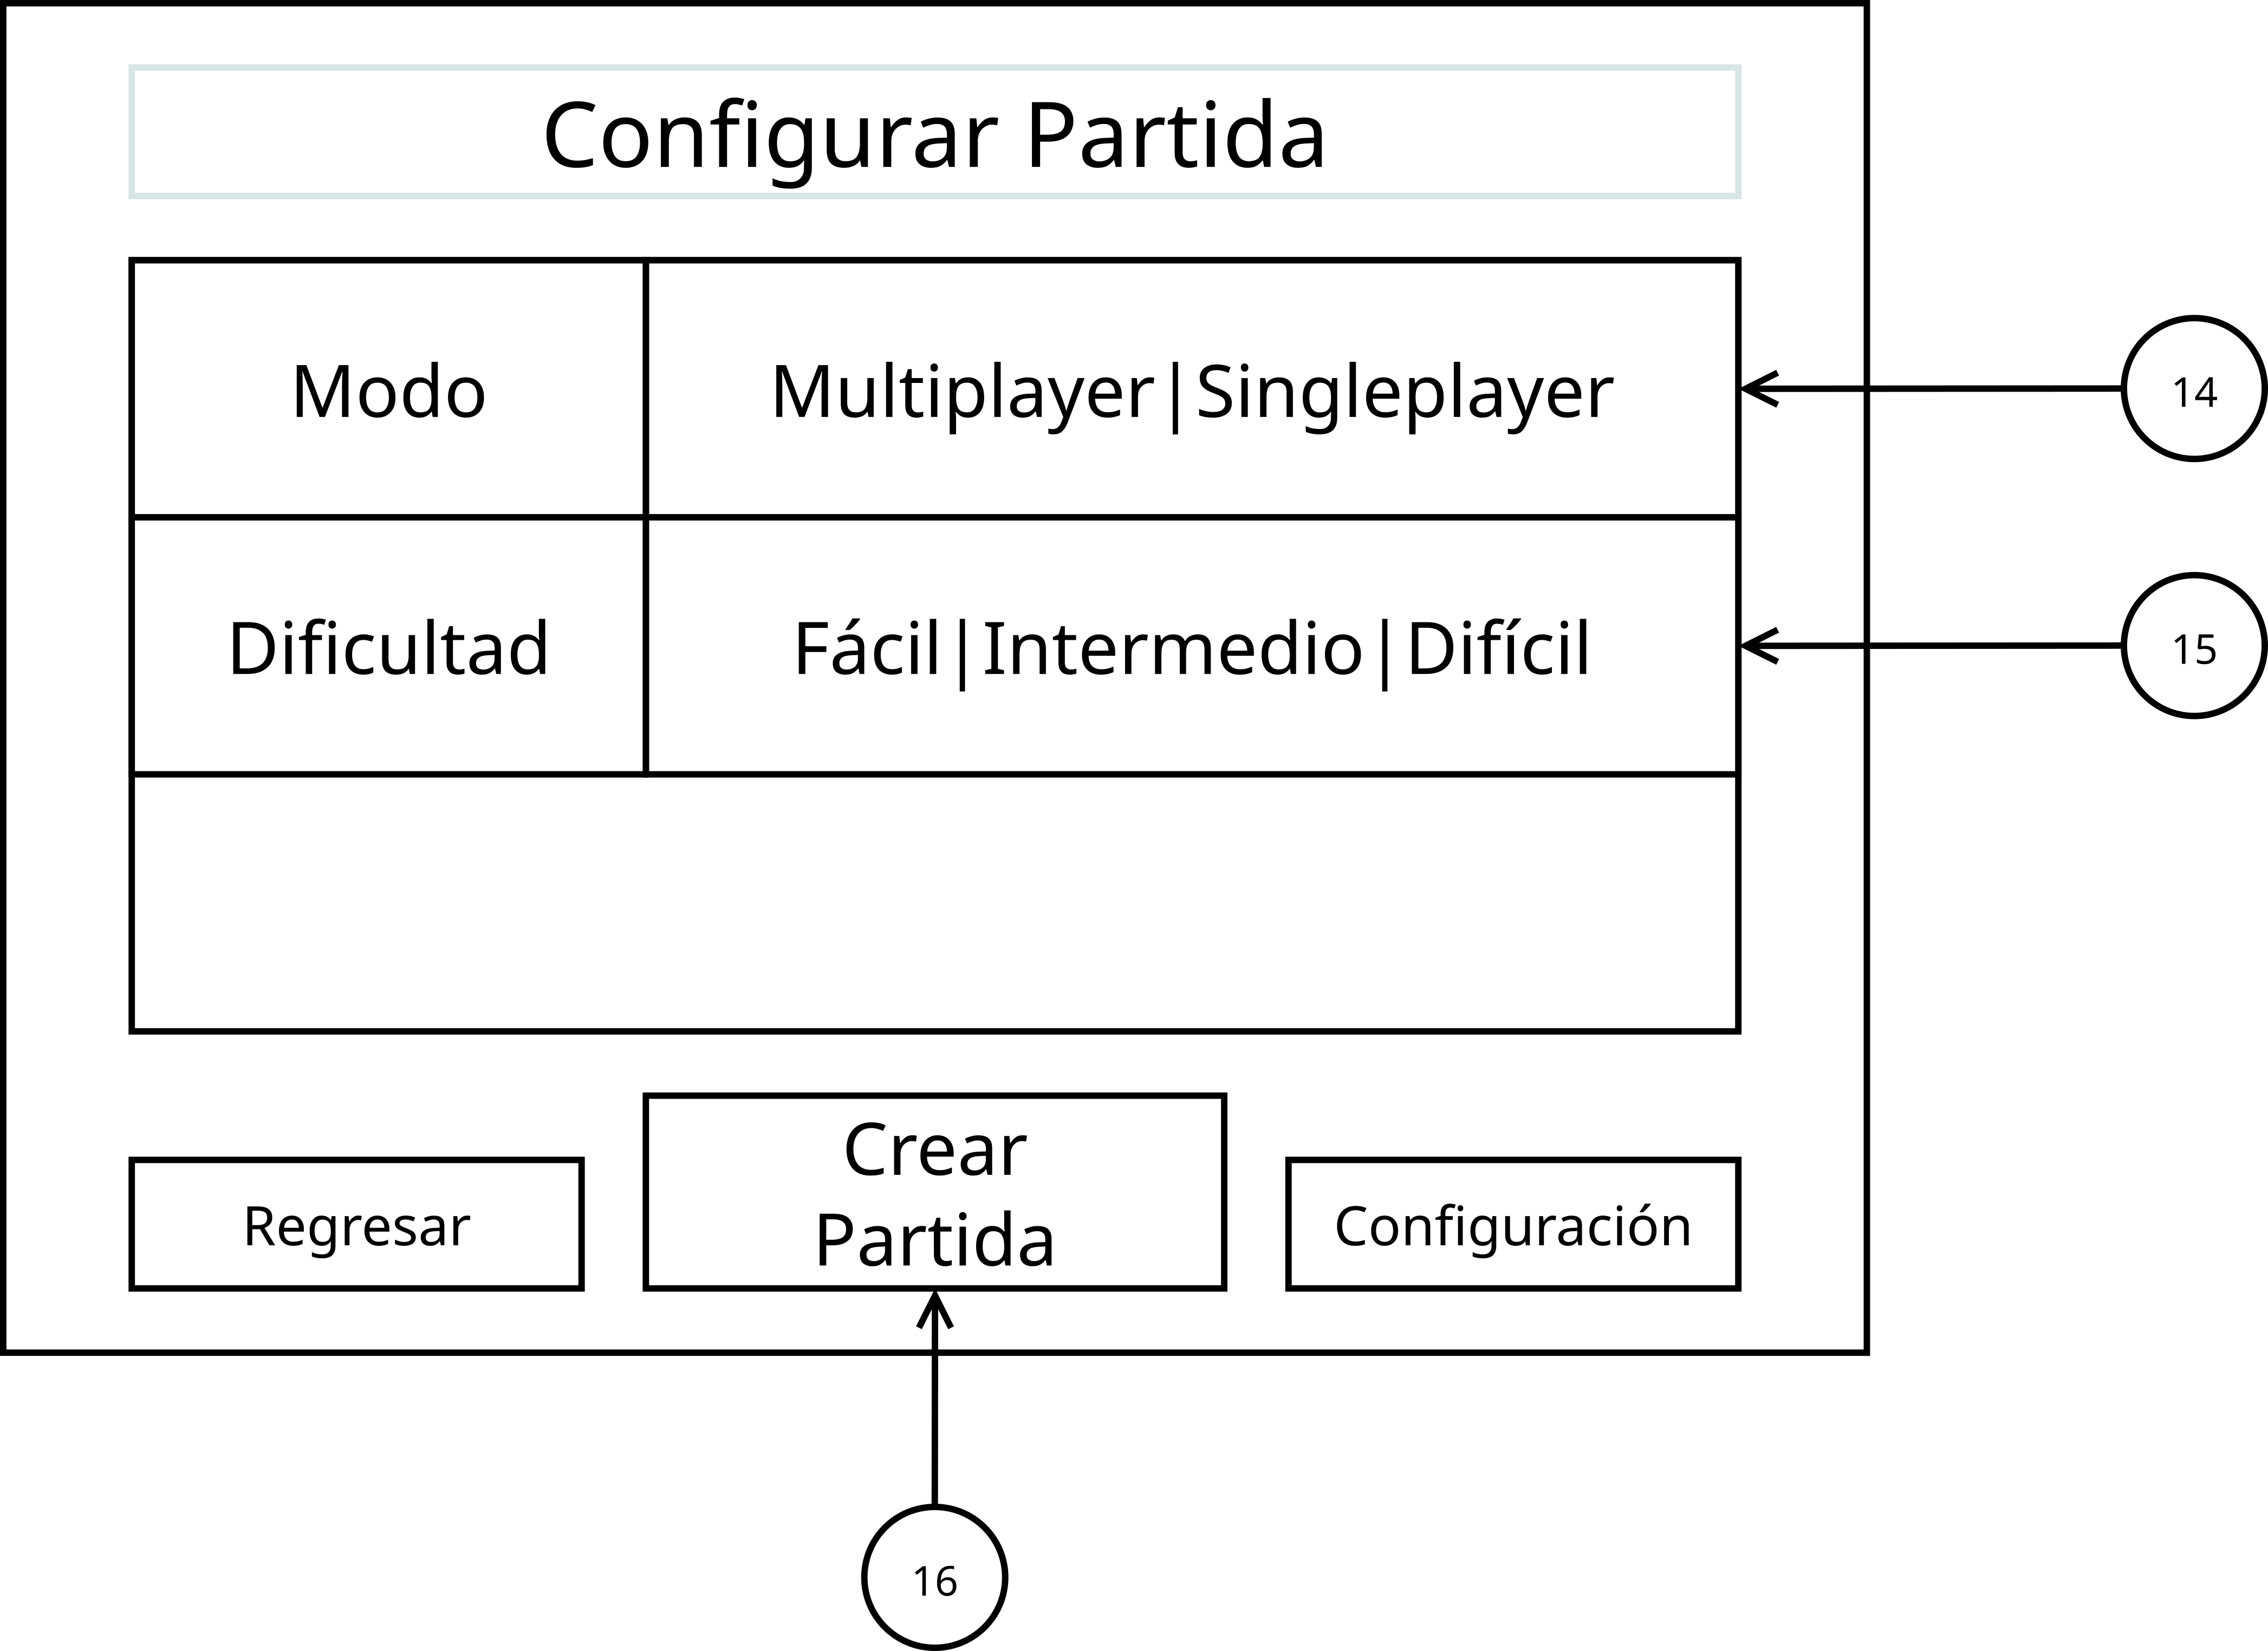
\includegraphics[width=0.6\textwidth]{5-Cuerpo/Chapter5/5.5/I4.png} %
    \caption{Interfaz del menú de configuración de partida}
    \label{fig:Interface_Configuracion_Partida}
\end{figure}
\begin{enumerate}\setcounter{enumi}{13}
    \item \textbf{Selector de modo}: Este selector permitirá especificar si se
    desea jugar una partida contra bots (singleplayer) o contra otros jugadores
    (multiplayer).
    \item \textbf{Selector de dificultad}: Este selector permitirá especificar
    la dificultad con la que se desea jugar.
    \item \textbf{Botón de creación de partida}: Una vez configurada la partida
    o simplemente dejado los valores por defecto de la configuración, este botón
    permitirá acceder al menú de selección de personaje y crear la partida.
\end{enumerate}

\subsubsection{Modo selección de personaje}
\begin{figure}[H]
    \centering
    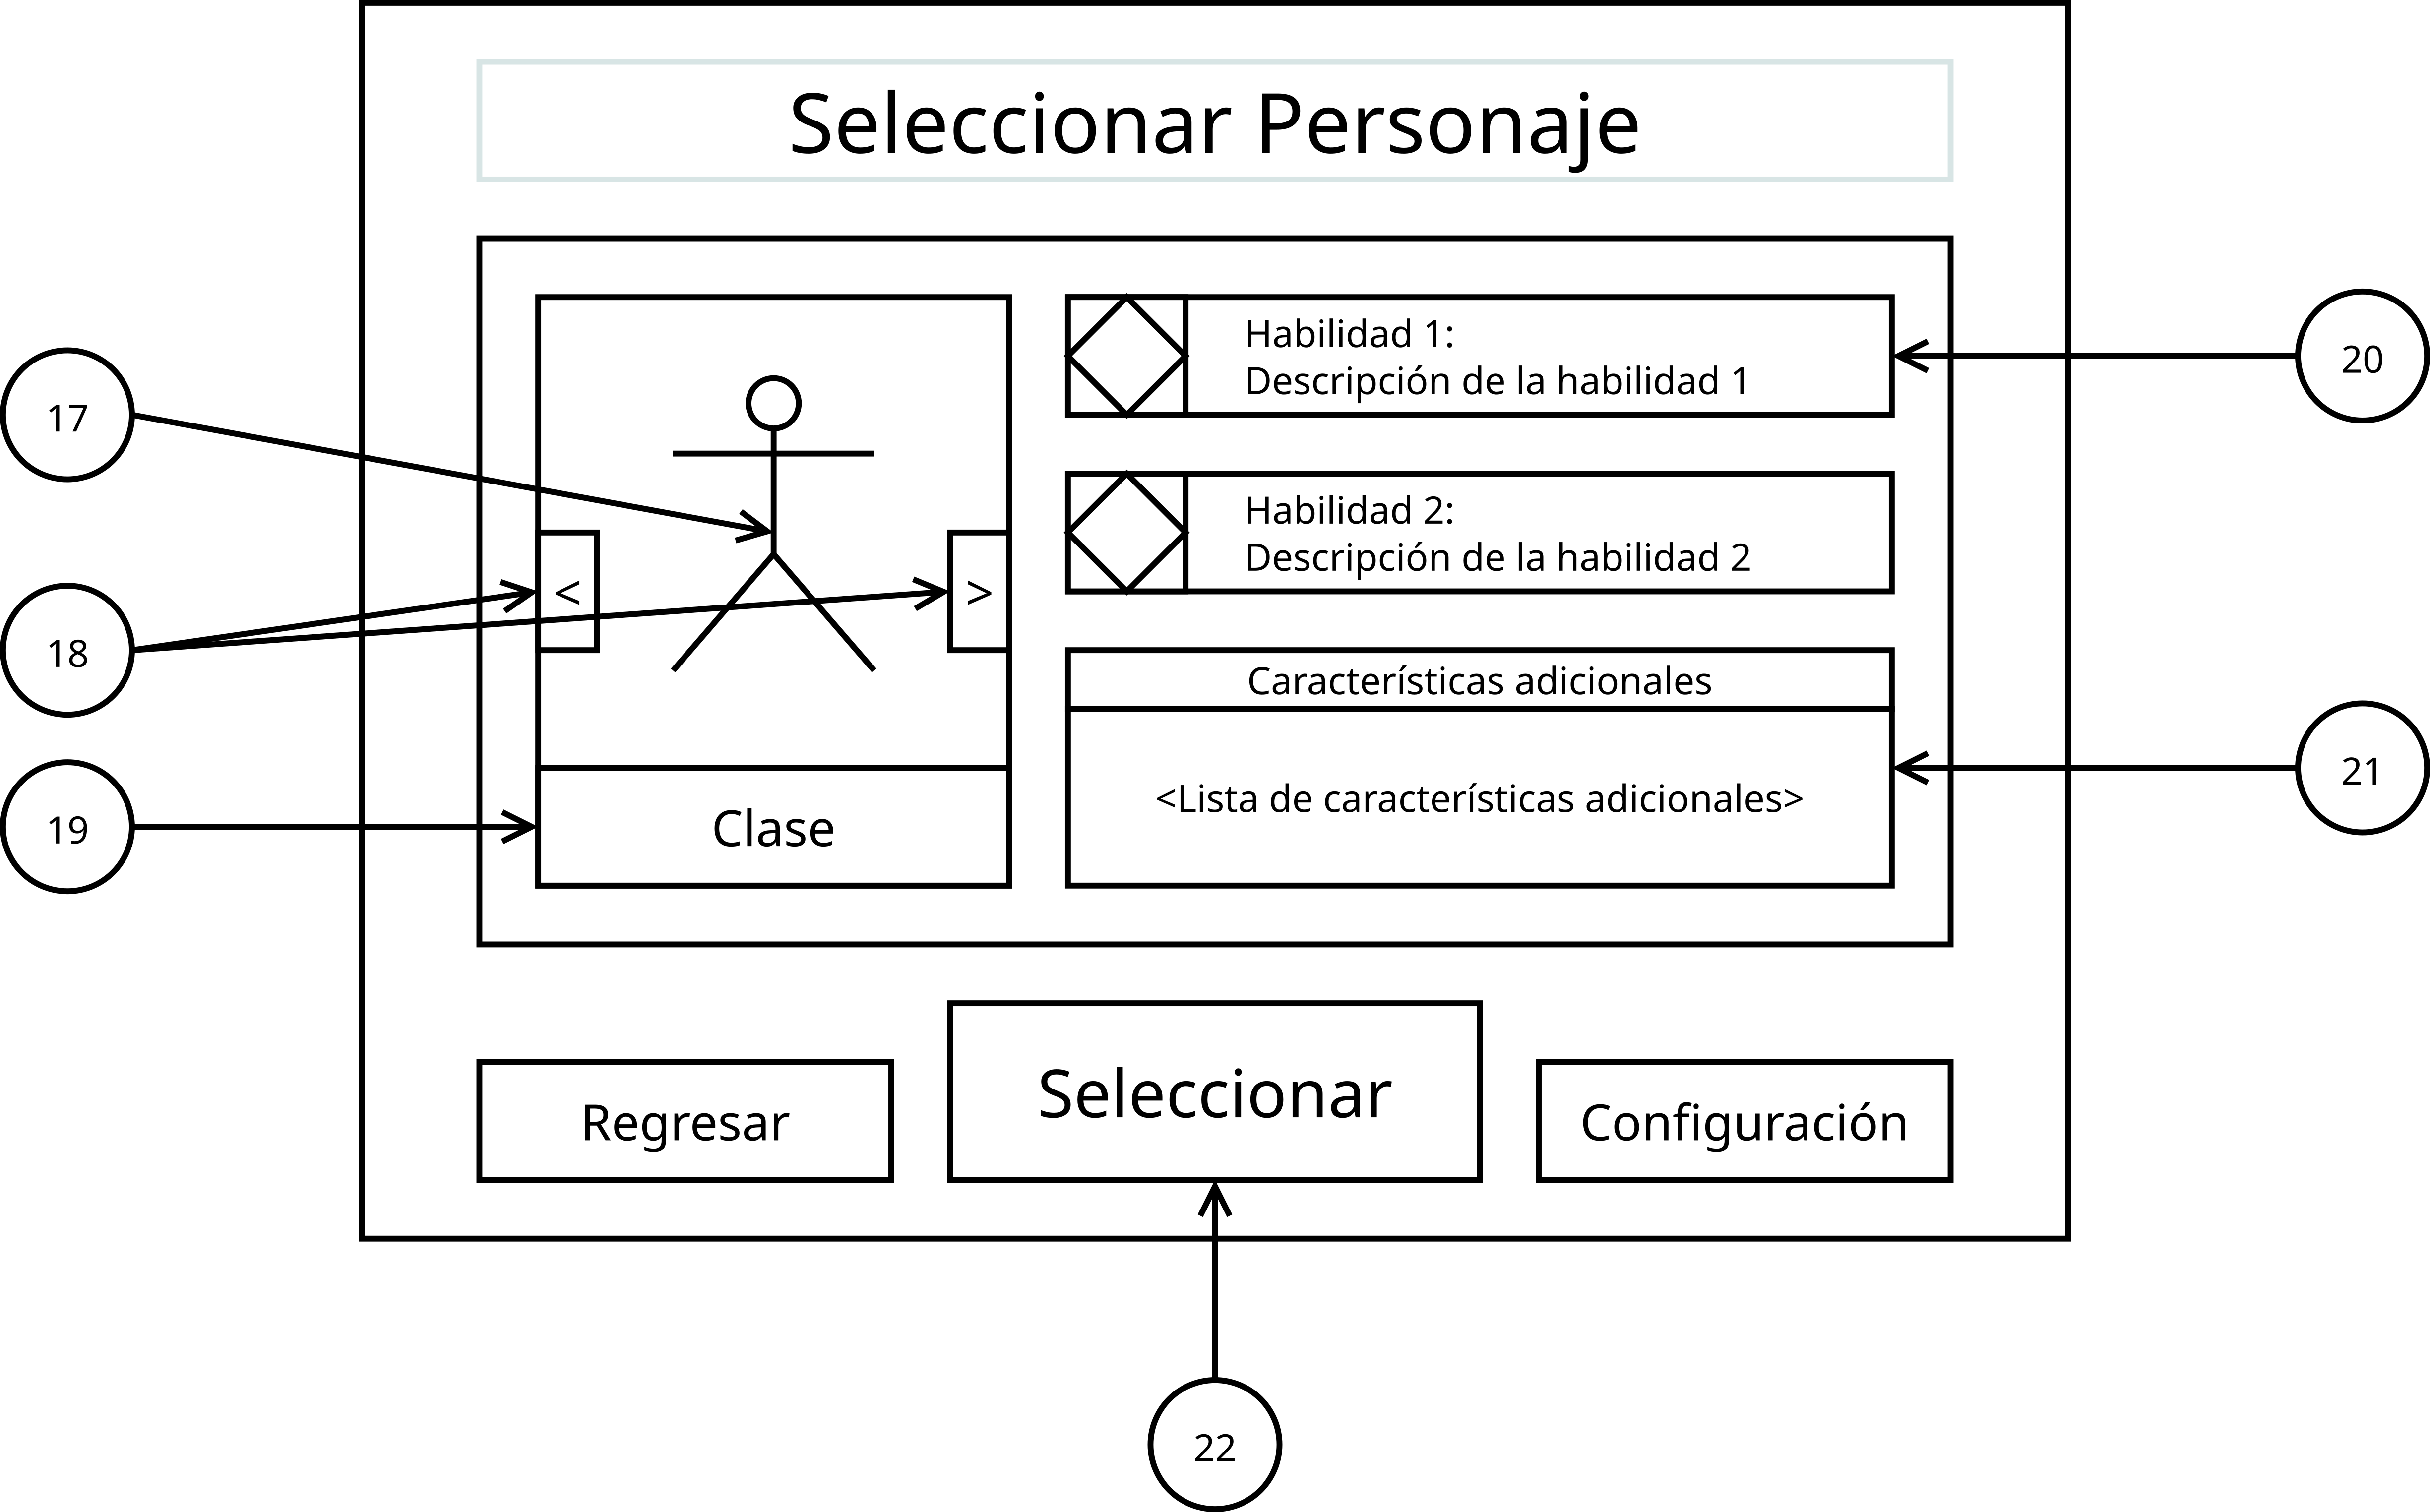
\includegraphics[width=0.6\textwidth]{5-Cuerpo/Chapter5/5.5/I5.png} %
    \caption{Interfaz del menú de selección de personaje}
    \label{fig:Interface_Seleccion_Personaje}
\end{figure}
\begin{enumerate}\setcounter{enumi}{16}
    \item \textbf{Vista del personaje}: Para facilitar la selección del
    personaje, se muestra en una ventana la forma y la estética de los
    personajes.
    \item \textbf{Botones de cambio de personaje}: El personaje actualmente
    visibile en la ventana de vista del personaje será el escogido para la
    partida, por tanto se necesitan estos botones para cambiar el personaje. Una
    vez llegado al último personaje o al primero, avanzar o retroceder
    respectivamente simplemente ciclará sobre la lista de personajes.
    \item \textbf{Clase del personaje}: Se mostrará también la clase del
    personaje.
    \item \textbf{Habilidad del personaje}: Cada personaje tendrá dos
    habilidades especiales que podrán verse desde estas ventanas para facilitar
    la selección del jugador.
    \item \textbf{Información adicional sobre el personaje}: Adicionalmente se
    mostrarán las diferencias que tiene el personaje en cuanto a estadísticas y
    valores internos en comparación a los demás.
    \item \textbf{Botón de selección}: Una vez decidido el personaje con el que
    se quiere jugar, se pulsará este botón para empezar la partida.
\end{enumerate}

\subsubsection{Modo partida}
\begin{figure}[H]
    \centering
    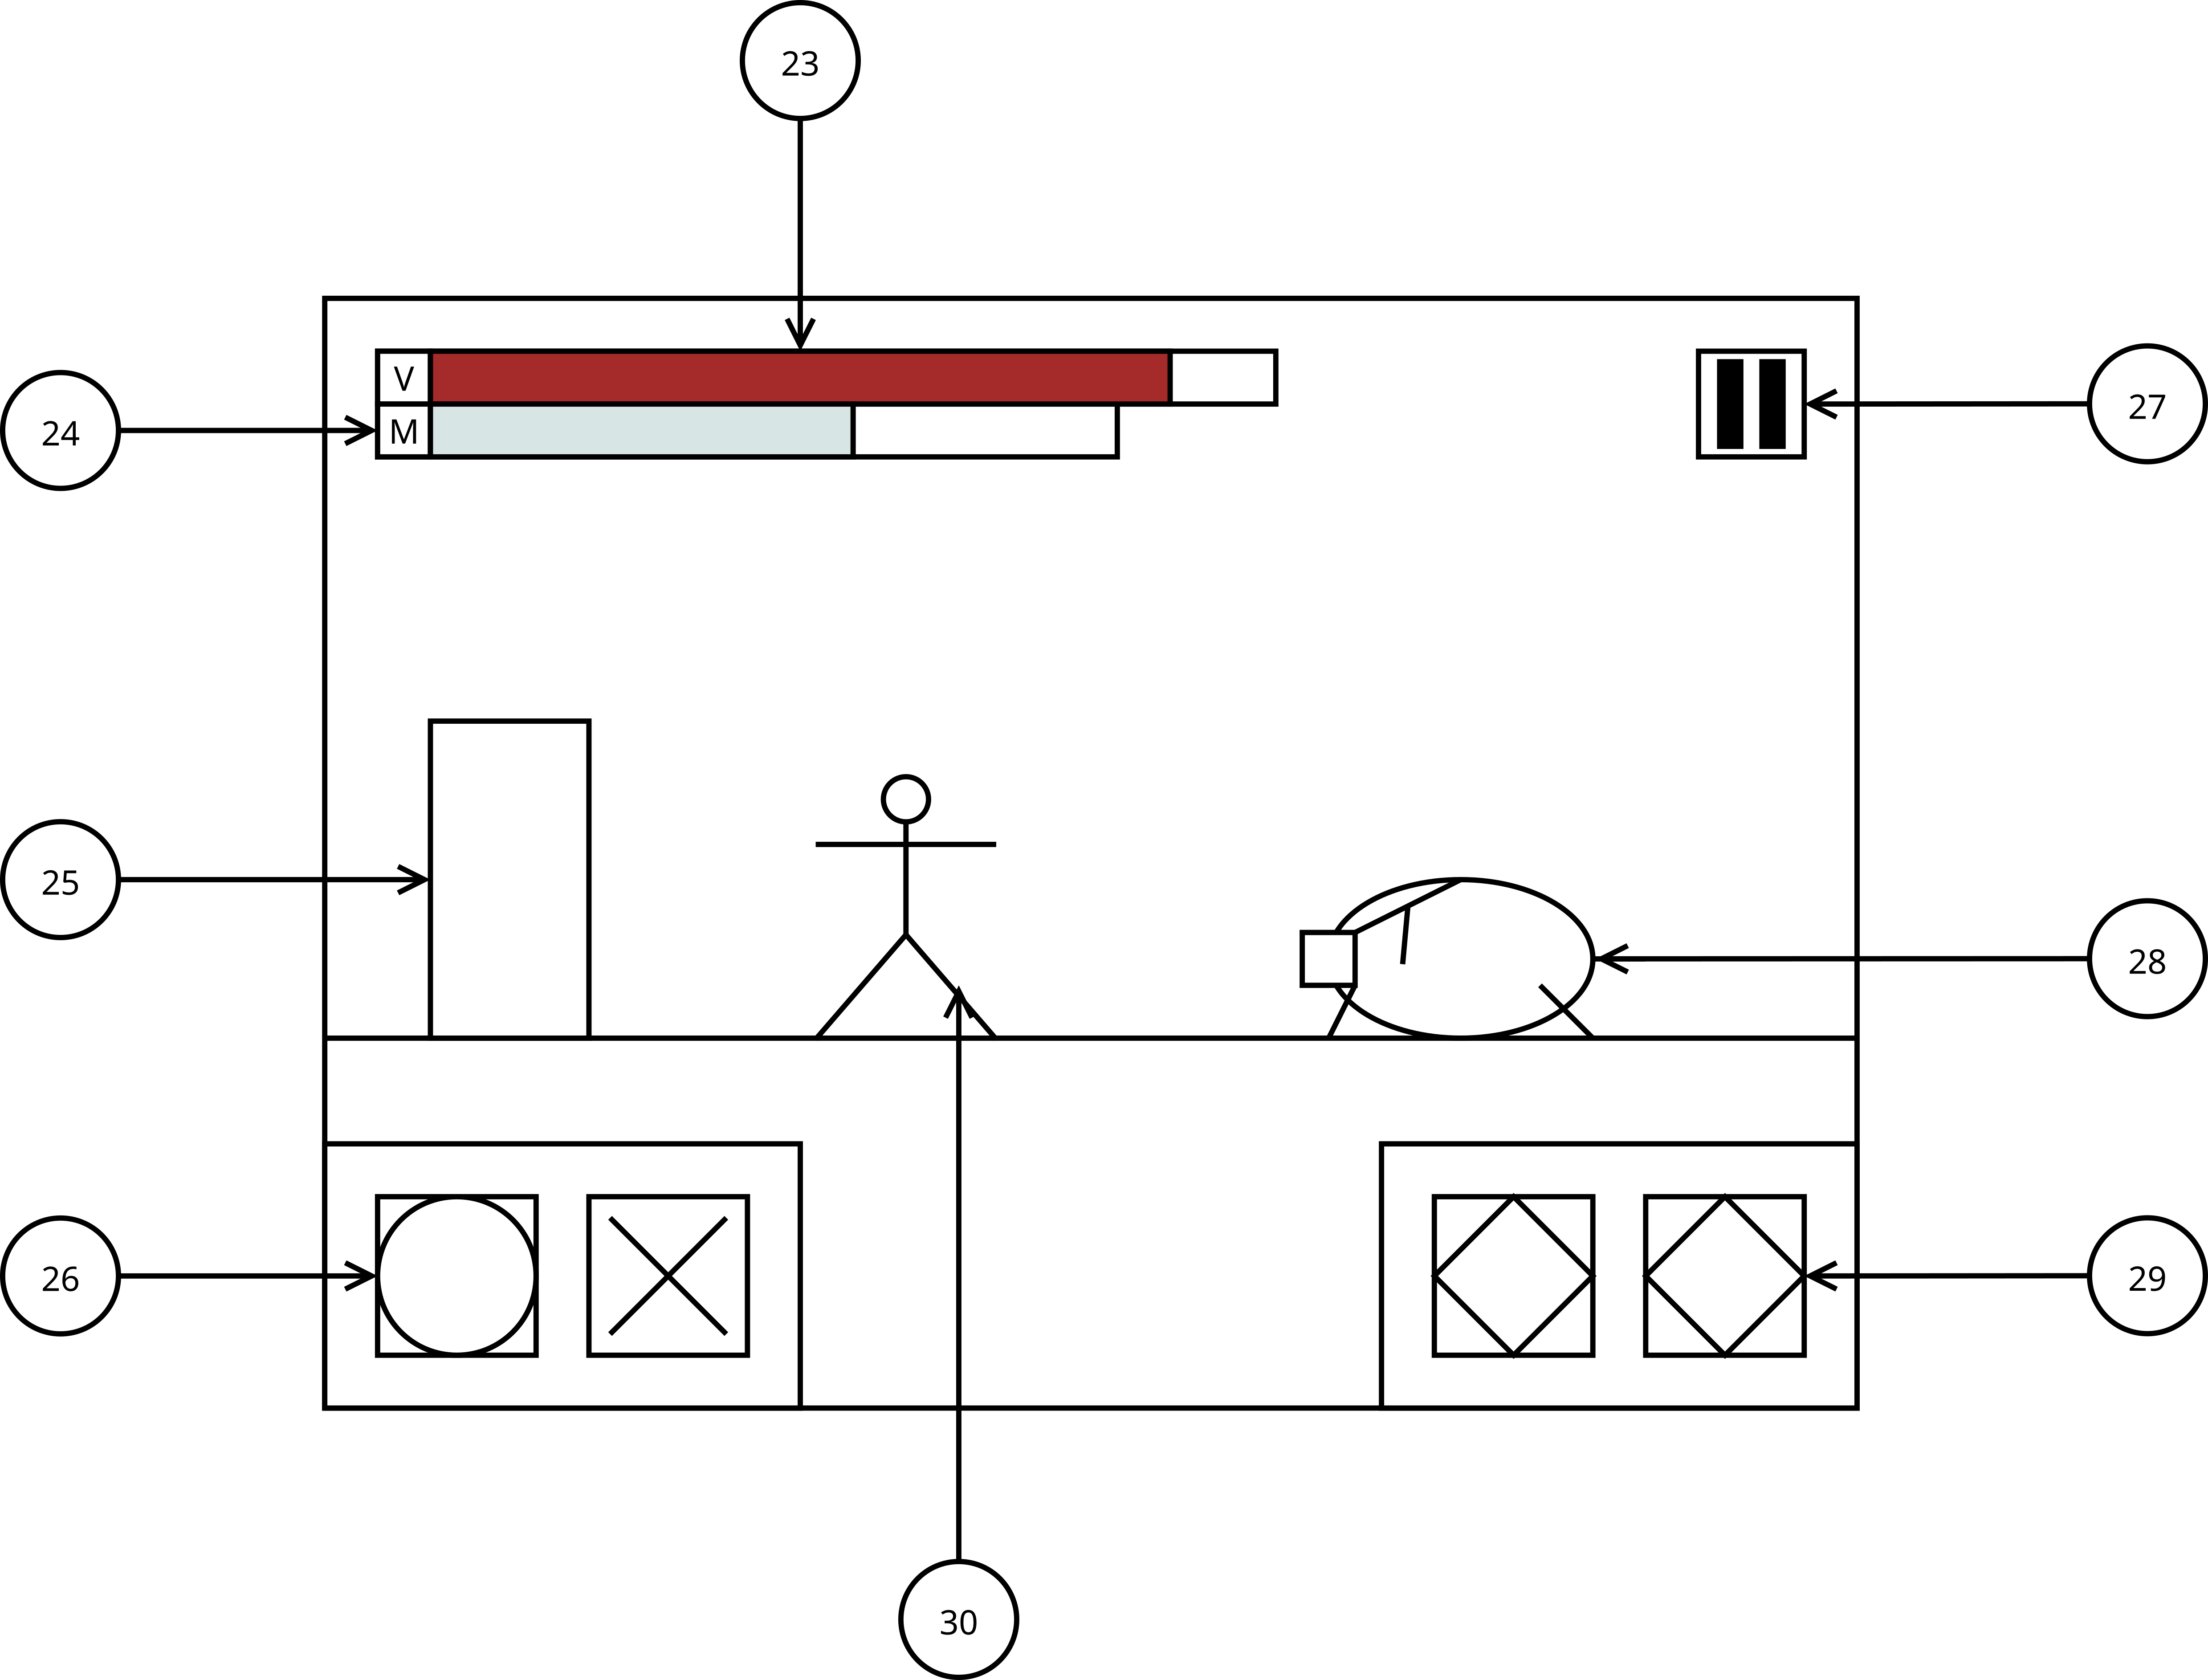
\includegraphics[width=0.6\textwidth]{5-Cuerpo/Chapter5/5.5/I6.png} %
    \caption{Interfaz de la partida}
    \label{fig:Interface_Partida}
\end{figure}
\begin{enumerate}\setcounter{enumi}{22}
    \item \textbf{Barra de vida}: La cantidad de vida o salud del personaje
    durante una partida se mostrará en esta barra, además de la cantidad máxima
    de vida que puede tener.
    \item \textbf{Barra de mana}: Así como con la barra de vida, esta barra
    muestra la cantidad de maná o magia que posee el personaje junto con su
    valor máximo.
    \item \textbf{Puerta}: Un personaje siempre empieza en una puerta
    de entrada y su objetivo es encontrar la puerta de salida del nivel lo antes
    posible.
    \item \textbf{Objeto mágico}: Cuando se recolecte un objeto mágico, se podrá
    ver éste en este espacio. Para usarlo bastará con pulsar sobre su imagen.
    \item \textbf{Botón de pausa}: Para poder entrar en el modo pausa durante la
    partida, se utilizará este botón.
    \item \textbf{Enemigo}: El personaje deberá enfrentarse a distintos enemigos
    durante los niveles.
    \item \textbf{Habilidad especial}: Cada personaje posee dos habilidades
    especiales que puede utilizar durante la partida. Para hacer uso de ellas
    deberá pulsar en su espacio respectivo después de haber esperado un tiempo
    de \emph{enfriamiento} o \emph{cooldown}.
    \item \textbf{Personaje}: El personaje seleccionado en el menú anterior será
    aquel que controlará el jugador durante la partida.
\end{enumerate}

\subsubsection{Modo pausa}
\begin{figure}[H]
    \centering
    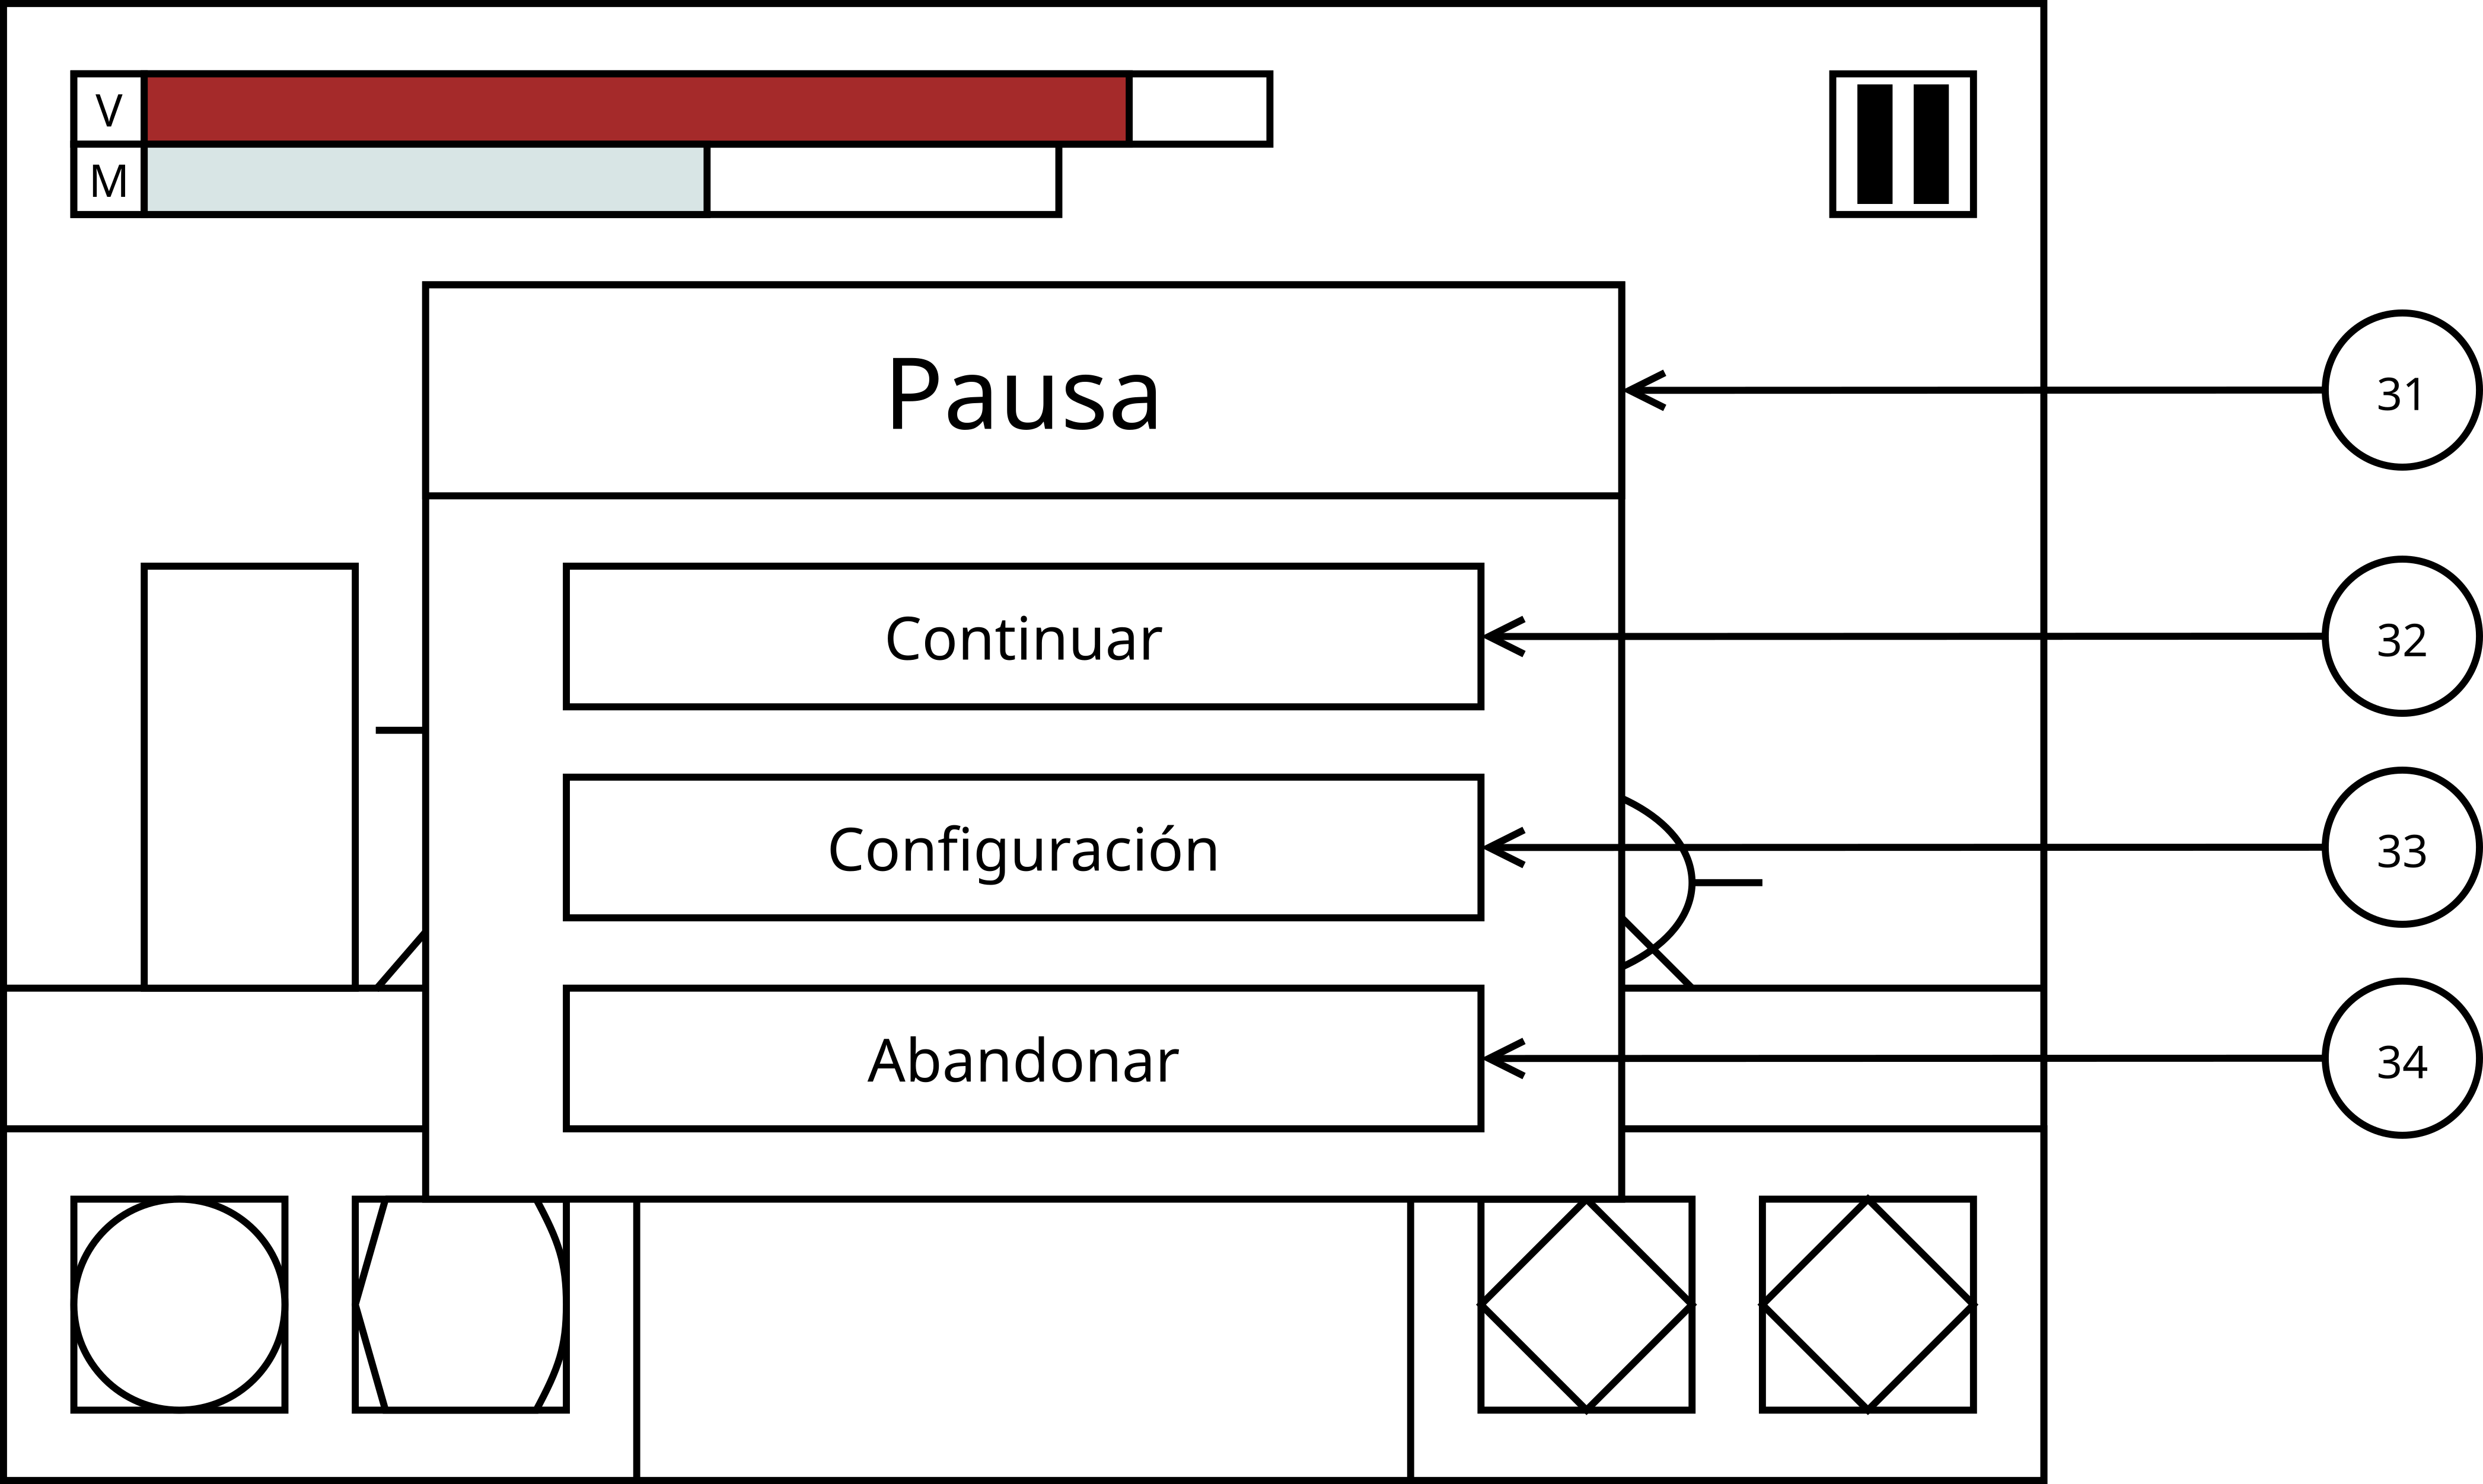
\includegraphics[width=0.6\textwidth]{5-Cuerpo/Chapter5/5.5/I7.png} %
    \caption{Interfaz del menú de pausa}
    \label{fig:Interface_Pausa}
\end{figure}
\begin{enumerate}\setcounter{enumi}{30}
    \item \textbf{Nombre del menú}: Se mostrará el nombre del menú que aparece
    en la partida.
    \item \textbf{Botón continuar}: Al pulsar este botón se saldrá del menú de
    pausa y se volverá a la partida.
    \item \textbf{Botón de configuración}: Al pulsar este botón se irá al menú
    de configuración general.
    \item \textbf{Botón abandonar}: Al pulsar este botón se abandonará la
    partida y se dará por perdida.
\end{enumerate}

\subsubsection{Modo victoria}
\begin{figure}[H]
    \centering
    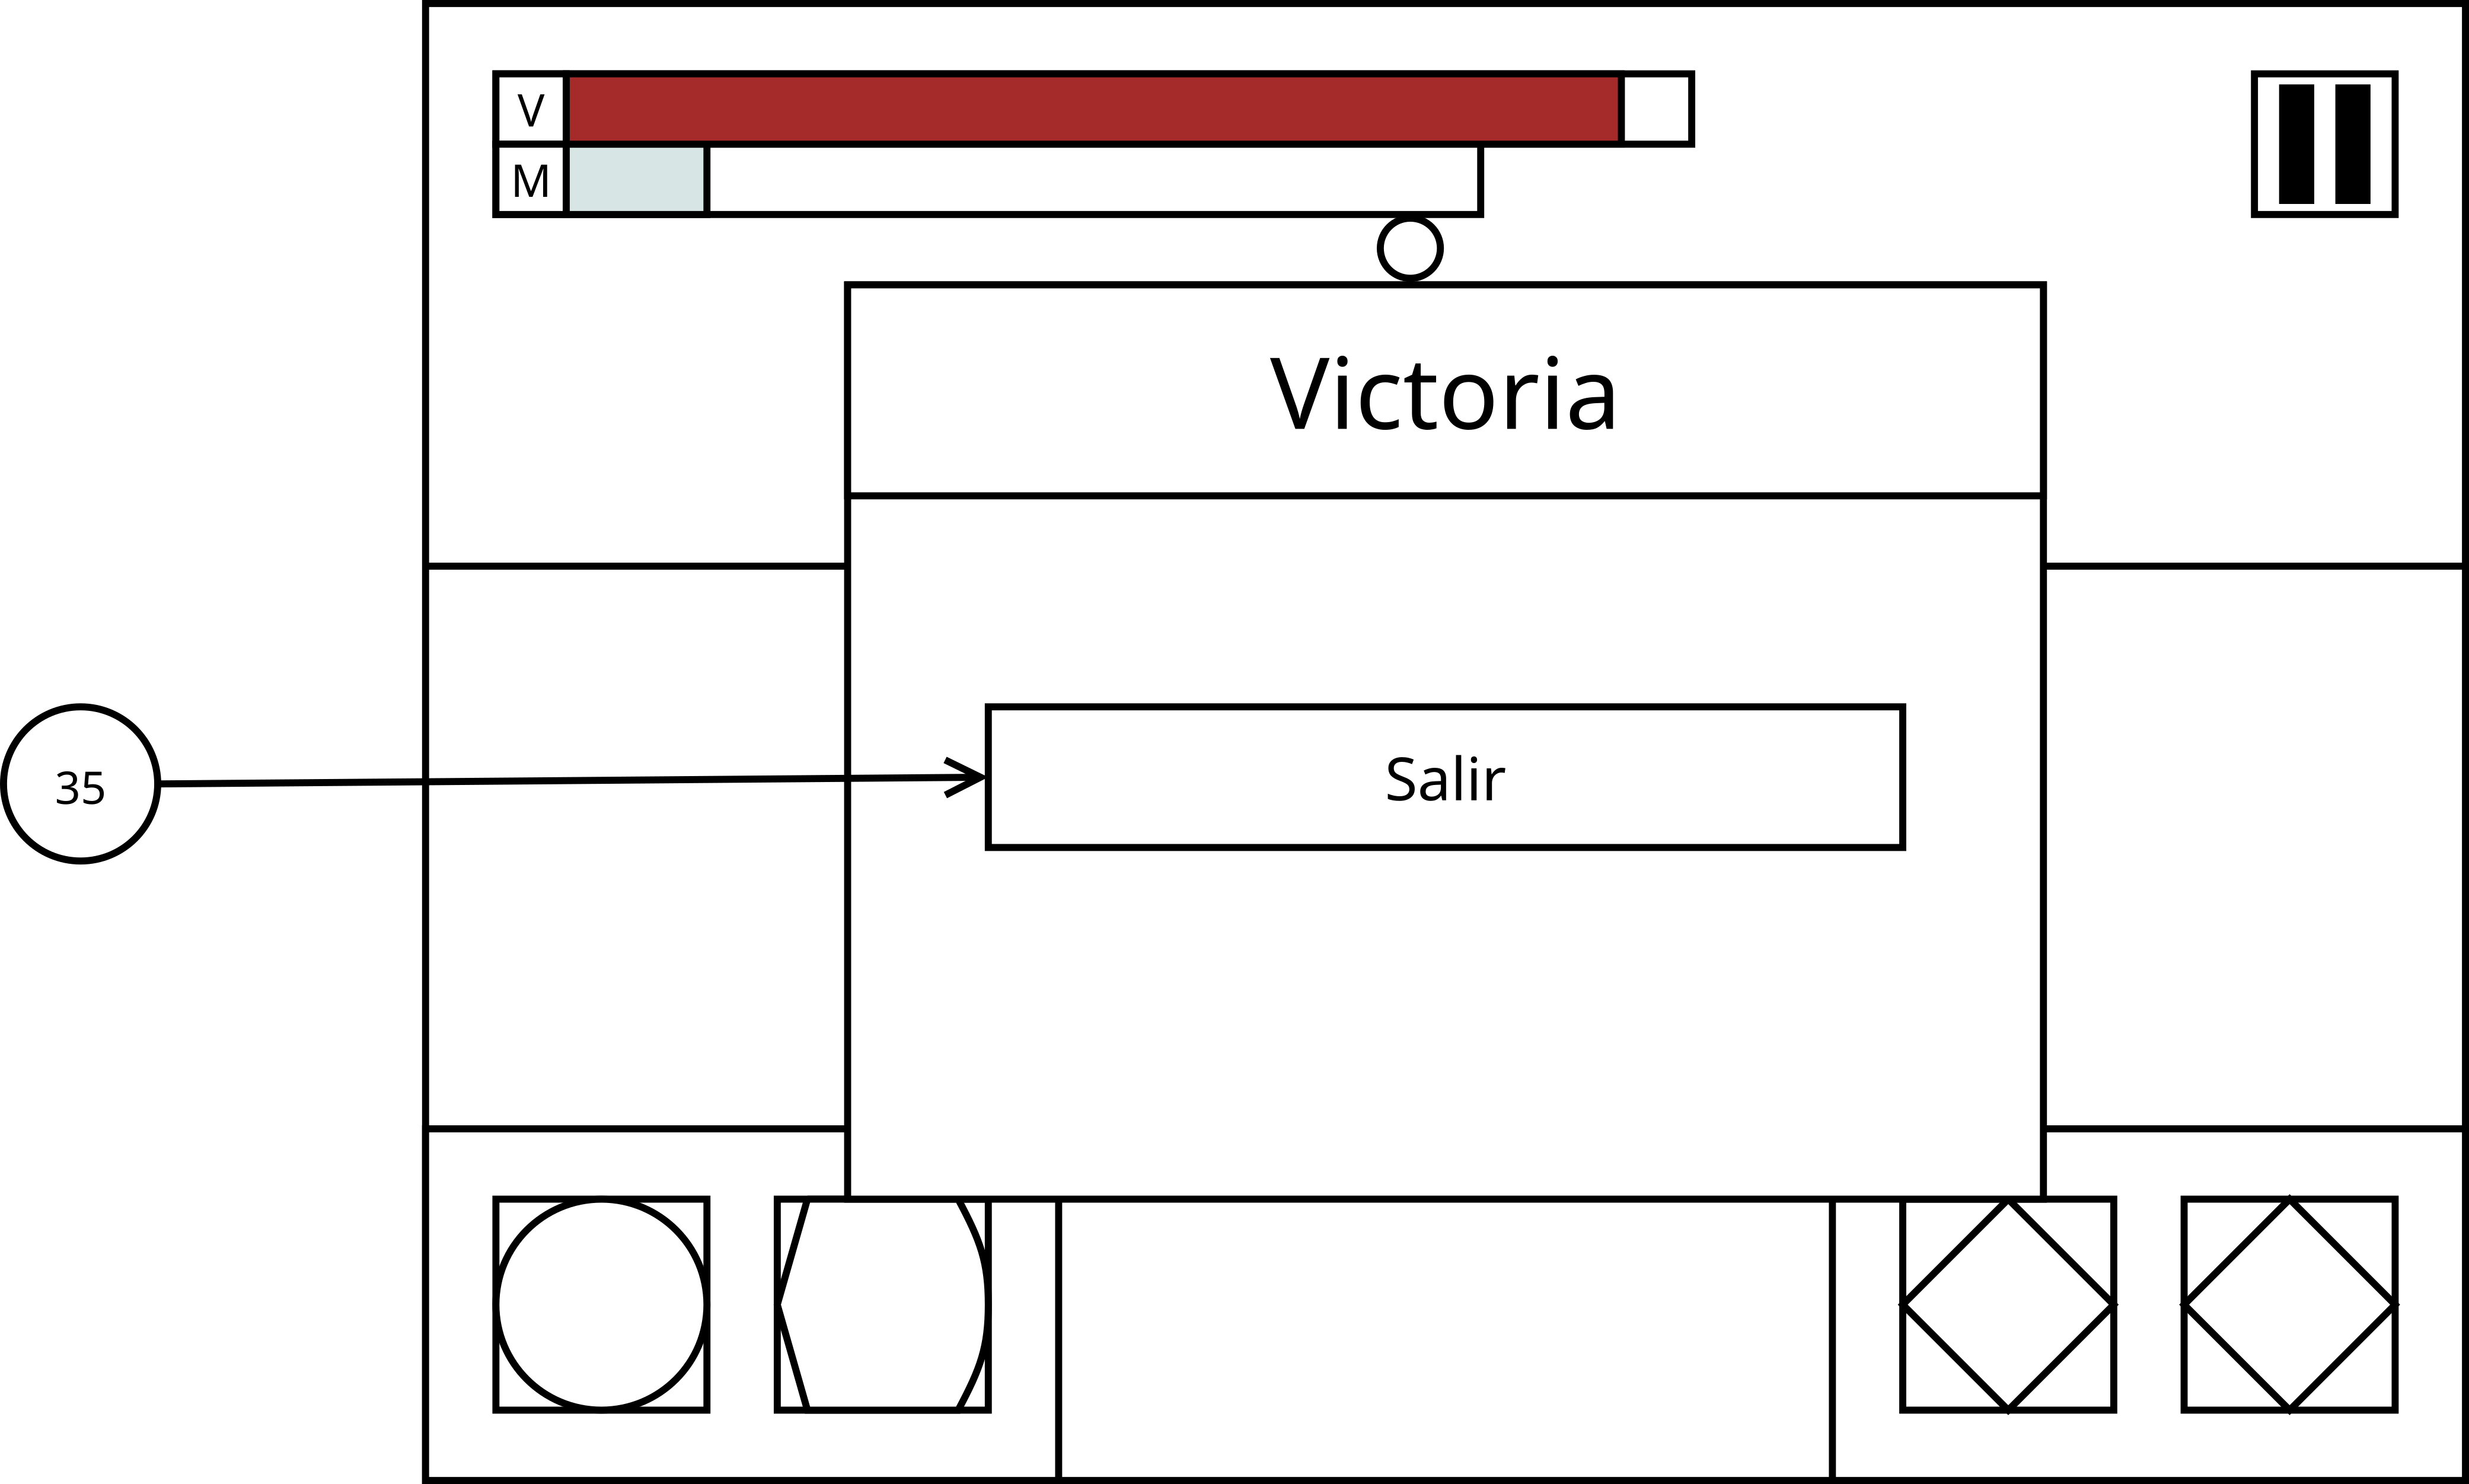
\includegraphics[width=0.6\textwidth]{5-Cuerpo/Chapter5/5.5/I8.png} %
    \caption{Interfaz del menú de victoria}
    \label{fig:Interface_Victoria}
\end{figure}
\begin{enumerate}\setcounter{enumi}{34}
    \item \textbf{Botón de salida}: La única posibilidad en el modo de victoria
    o derrota es salir de la partida al modo perfil.
\end{enumerate}

\subsubsection{Modo derrota}
\begin{figure}[H]
    \centering
    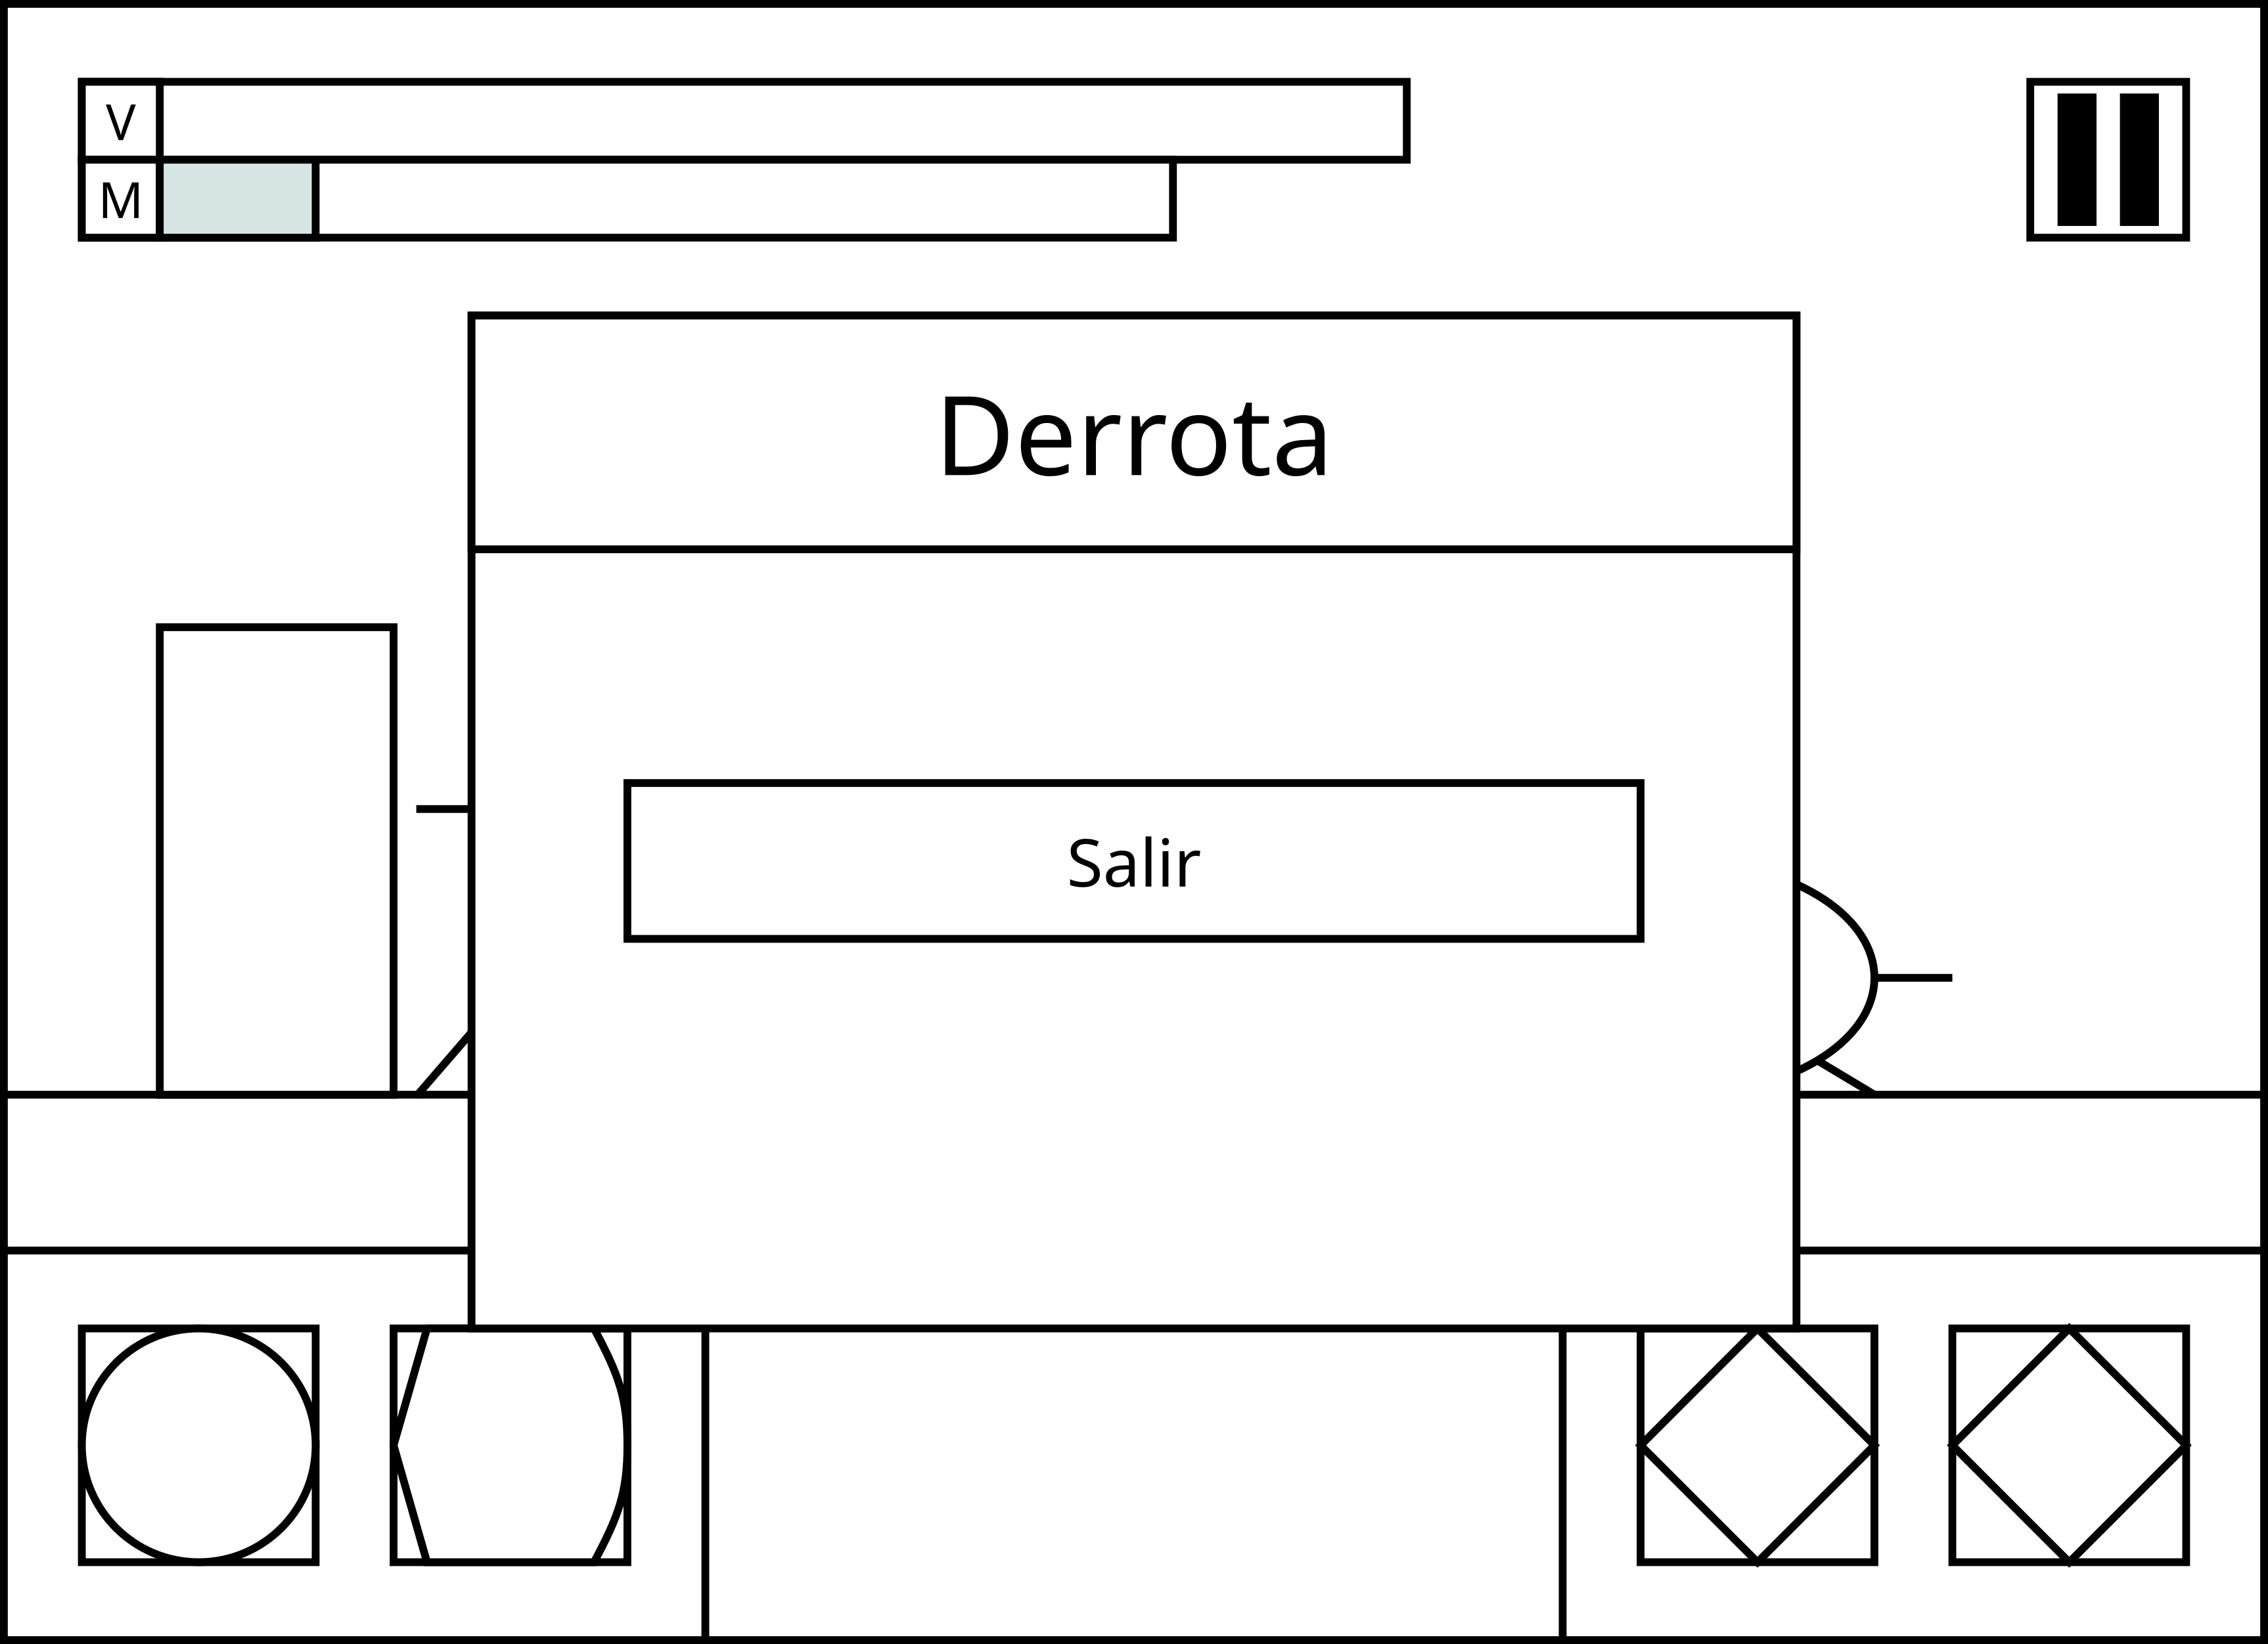
\includegraphics[width=0.5\textwidth]{5-Cuerpo/Chapter5/5.5/I9.png} %
    \caption{Interfaz del menú de derrota}
    \label{fig:Interface_Derrota}
\end{figure}


\subsubsection{Modo configuración general}
\begin{figure}[H]
    \centering
    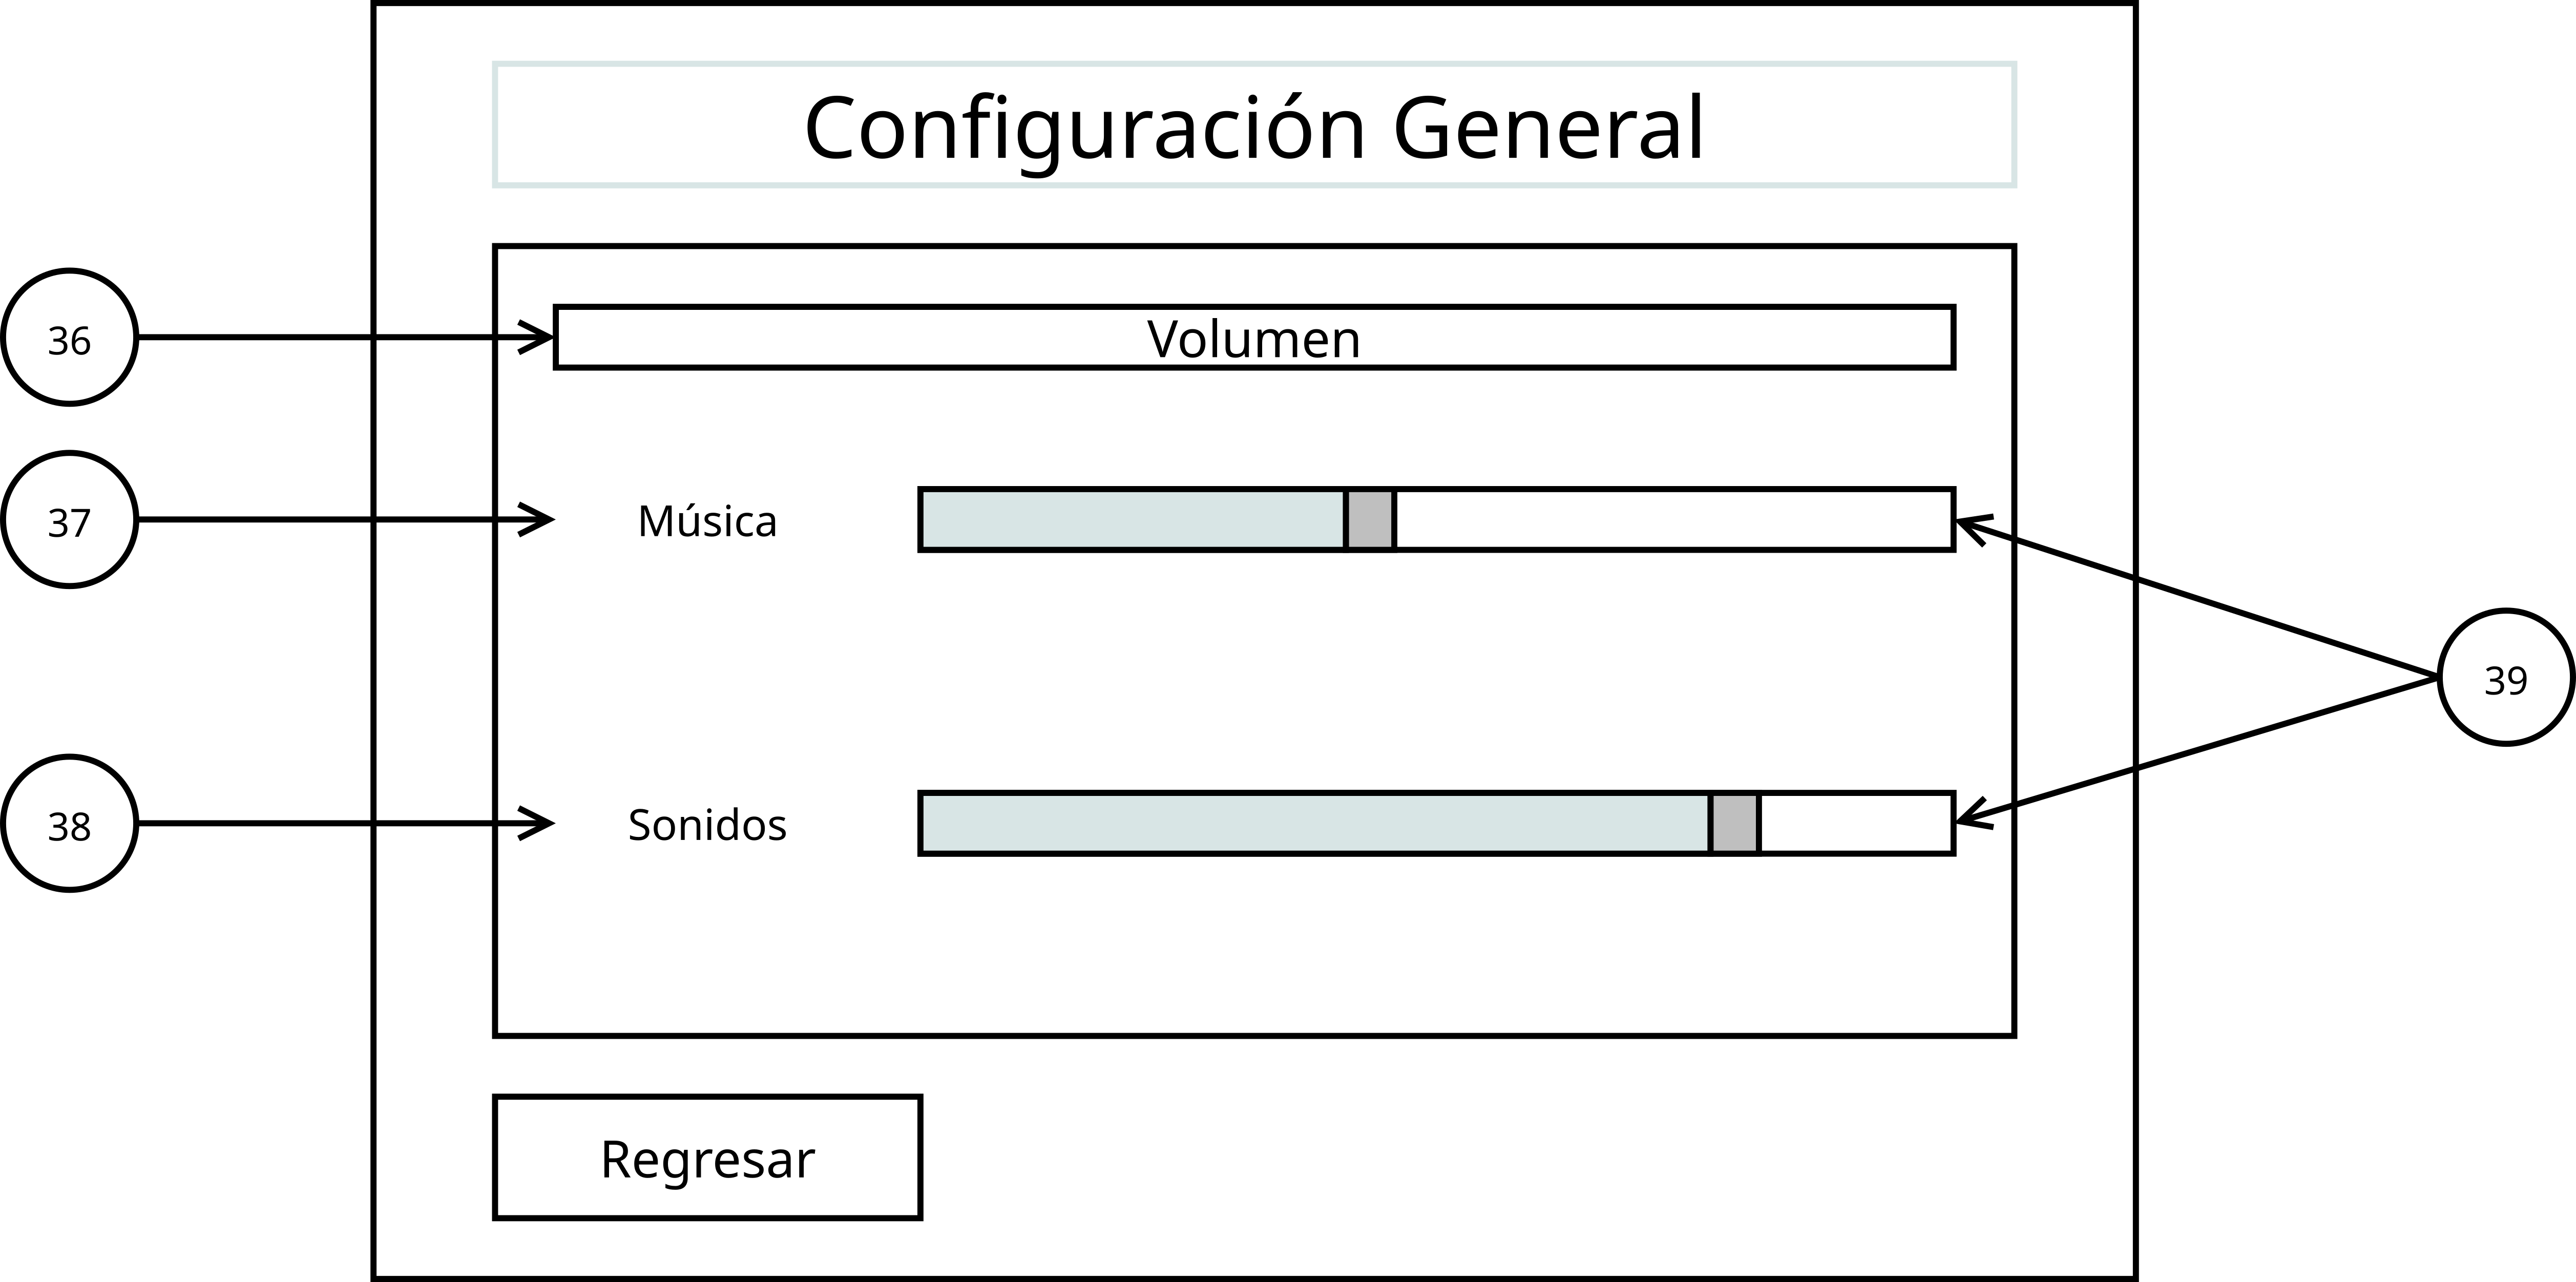
\includegraphics[width=0.6\textwidth]{5-Cuerpo/Chapter5/5.5/I10.png} %
    \caption{Interfaz del menú de configuración general}
    \label{fig:Interface_Configuracion_General}
\end{figure}
\begin{enumerate}\setcounter{enumi}{35}
    \item \textbf{Nombre de sección de configuración}: Dentro de la
    configuración general se tendrá una serie de configuraciones que se podrán
    agrupar en distintas categorías.
    \item \textbf{Volumen de la música}: El control del volumen de la música.
    \item \textbf{Volumen de los sonidos}: El control del volumen de los efectos
    de sonido.
    \item \textbf{Barras de control de volumen}: Las barras que controlan como
    tal el volumen del sonido del juego.
\end{enumerate}